%!TEX root = ../Report.tex
\chapter{Implementação}
\label{chp:implement}
Esta secção apresenta a implementação das ferramentas acima mencionadas e a forma como estas foram utilizadas no contexto do projeto, desde a sua interação com outras ferramentas até aos seus benefícios para a solução. As seguintes subseções falam, em primeiro lugar, da camada de dados e como esta está organizada de modo a suportar o armazenamento de dados necessitado para o projeto.\newline\\
Em segundo lugar, descreve a camada de processamento e como a comunicação e a troca de dados é feita entre as várias secções da plataforma, como por exemplo, entre o frontend e a base de dados.\newline\\
Por fim descreve o frontend e como este está estruturado de modo a cumprir os objetivos que foram definidos para o projeto e também fala acerca dos nós/APUs, como estes estão configurados e como eles são acedidos e reconfigurados pelo utilizador da plataforma que pretende realizar experiências.

\section{Camada de dados}
Nesta secção vamos discutir com detalhe a implementação da camada de dados. Em primeiro lugar, demonstramos o modelo de dados da base de dados.\newline
No bloco dos utilizadores, temos as seguintes tabelas:
\begin{itemize}
    \item \textbf{Profile} – esta tabela modela um utilizador e as suas informações;
    \item \textbf{Experience} – esta tabela modela uma experiência como por exemplo a sua data de início e de fim;
    \item \textbf{APU\_Config} - define a configuração a fornecer a APU para uma dada experiência;
    \item \textbf{APU} – tabela que contém a informação acerca de cada APU da rede como por exemplo o IP;
    \item \textbf{Role} – cada utilizador pode ser de vários roles como por exemplo “Advanced” e “Beginner”
\end{itemize}
\begin{figure}[!ht]
    \centering
    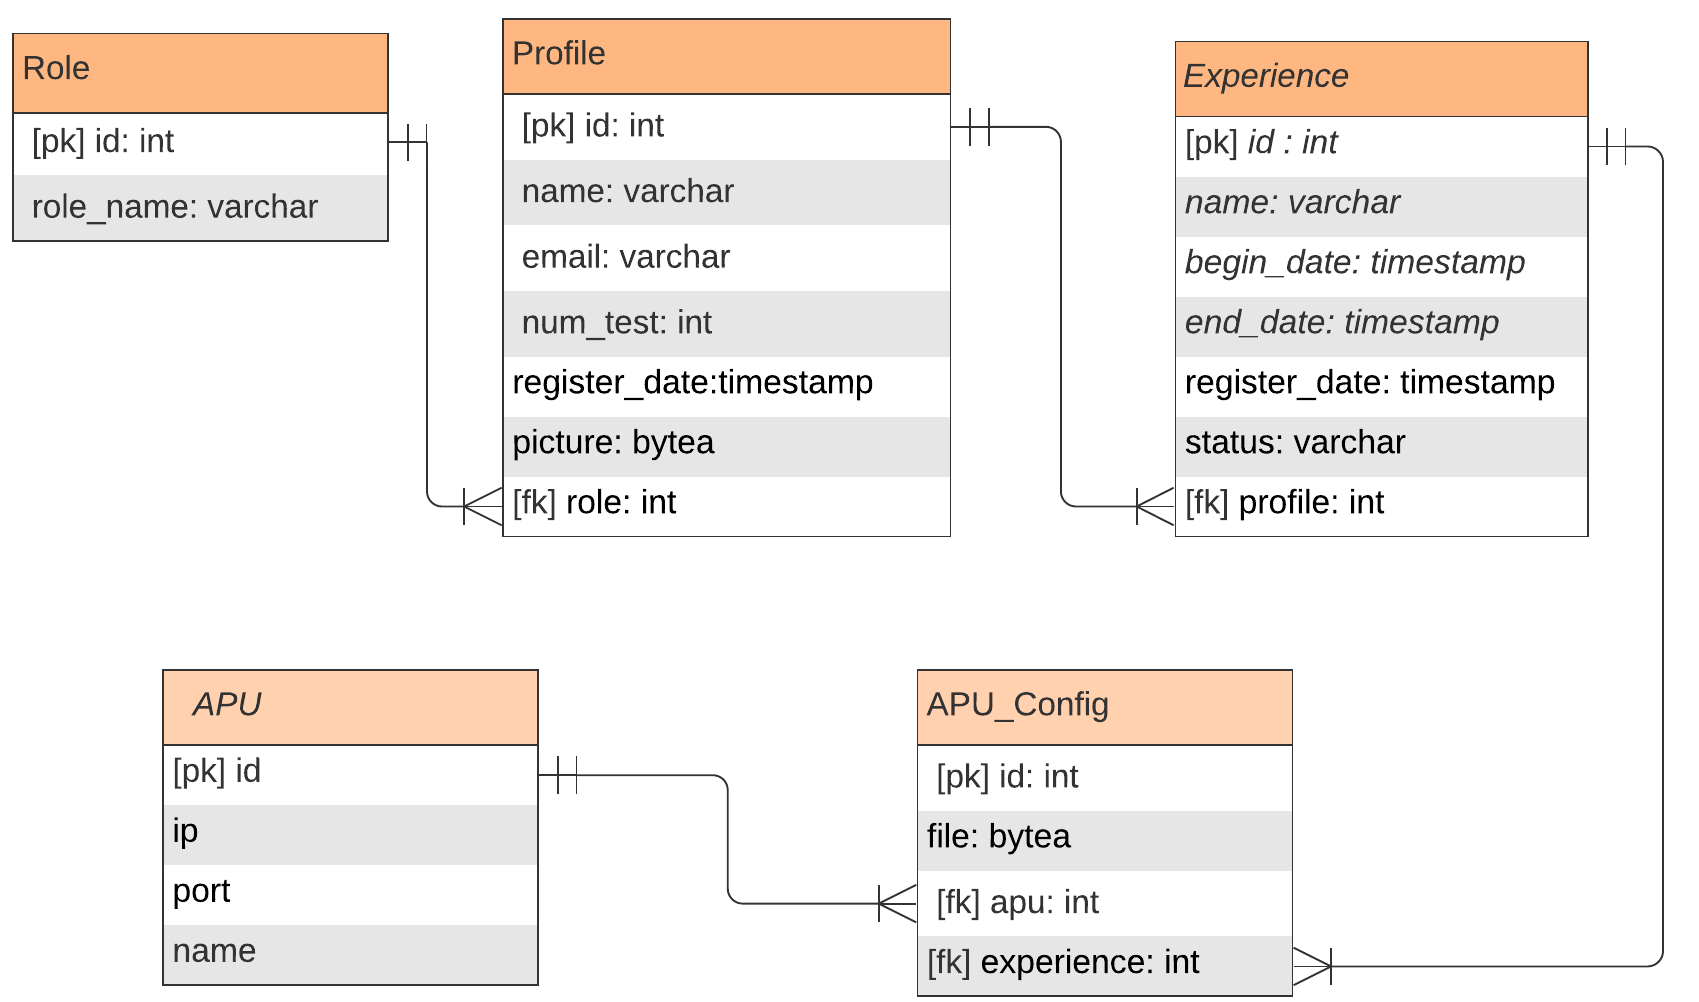
\includegraphics[width=0.75\textwidth, height=0.347\textheight]{images/data_model.png}
    \caption{Modelo de dados (bloco do utilizador)}
    \label{fig:dataModel}
\end{figure}
\section{Camada de processamento}
Esta secção apresenta o servidor principal da plataforma construído utilizando a framework Flask. Esta camada é responsável pela gestão do sistema, prover e receber dados do FrontEnd, consumir e atualizar a base de dados. Além de interagir com a Base de Dados, esta camada também interage com as APUs, inicializando automaticamente experiências e atuando como um proxy para disponibilizar informações das APUs em tempo real.\newline\\
Em termos de segurança, a maioria dos caminhos encontram-se protegidos.Como tal, requerem a adição de um JWT no header do pedido HTTP. Os utilizadores devem estar autenticados como utilizadores registados e/ou administradores. Os utilizadores normais podem apenas atualizar os dados associados a eles próprios, visualizar as experiências agendadas e ver os resultados das suas experiências anteriores. Os administradores, por sua vez, têm acesso à edição e visualização de toda a plataforma, inclusivé adicionar, atualizar e remover utilizadores, funções e APUs.
\newpage
\begin{figure}[!ht]
    \centering
    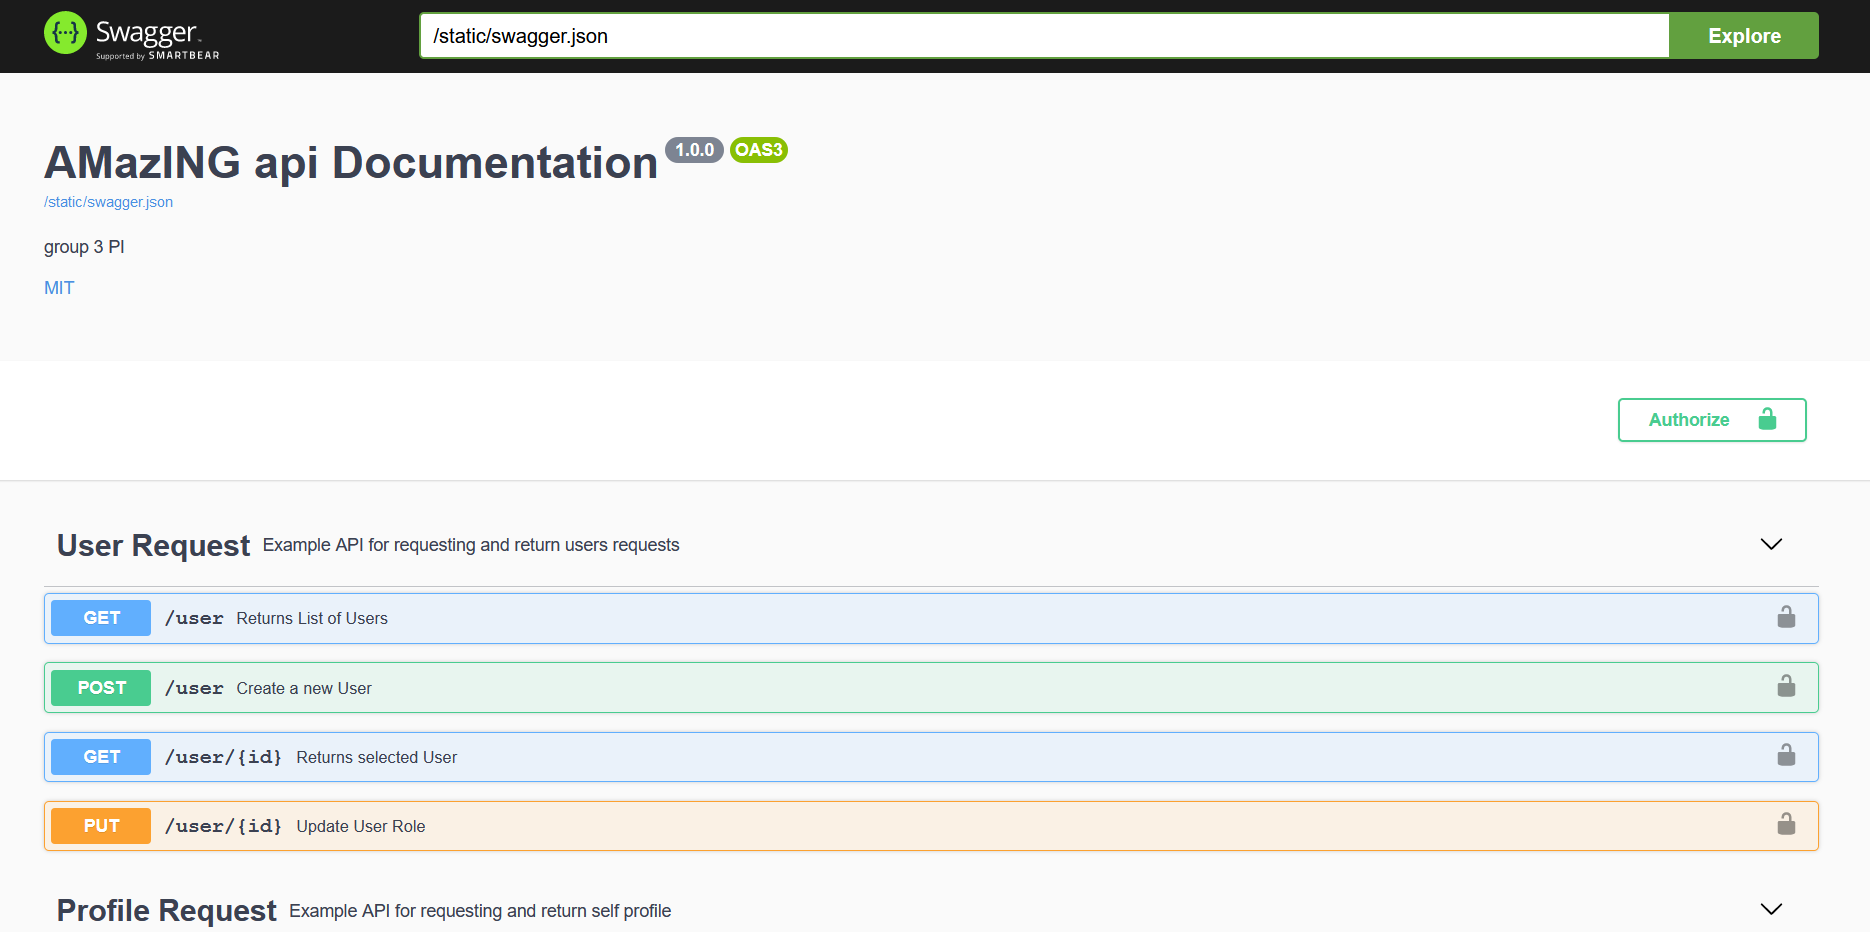
\includegraphics[width=0.9\textwidth]{images/swagger.png}
    \caption{Fragmento da documentação do Servidor utilizando o swagger}
    \label{fig:swagger}
\end{figure}

\section{Fluxo de dados}
Esta secção contém os fluxos de informação que passam ou se iniciam pelo servidor. De forma mais abrangente, os seguintes métodos utilizam a interface do SQLAlchemy para realizar operações do tipo CRUD.\newline
Começando pelos pedidos do tipo GET, ilustrado na figura, estes métodos obtêm a informação da base de dados, retornando, assim, a informação necessária, já tratada, de acordo com o caminho que é chamado.
Este tipo de operação não provoca alterações na informação guardada na base de dados, apenas obtém a mesma.
\begin{figure}[!ht]
    \centering
    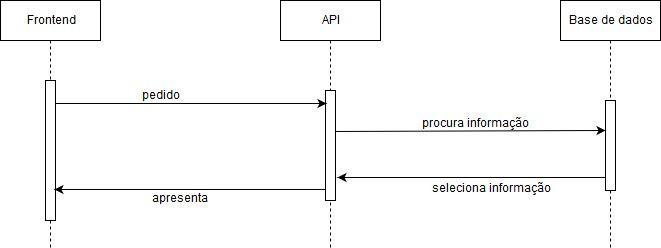
\includegraphics[width=0.9\textwidth]{images/fluxo1.jpg}
    \caption{Fluxo de comunicação para o método GET}
    \label{fig:get}
\end{figure}
\hfill\break
No que se concerne aos métodos POST, PUT e DELETE é realizado um pedido à API consoante o caminho necessário e são efetuadas ações sobre os dados guardados. É de salientar que estes três verbos da API têm funções diferentes:
\begin{itemize}[noitemsep]
    \item \textbf{PUT} - Alteração de Informações já existentes
    \item \textbf{POST} - Adição de novas informações
    \item \textbf{DELETE} - Apagar informações existentes
\end{itemize}
\begin{figure}[!ht]
    \centering
    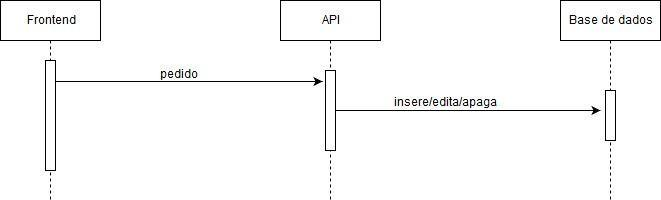
\includegraphics[width=0.8\textwidth]{images/fluxo2.jpg}
    \caption{Fluxo de comunicação para os métodos POST, PUT e DELETE}
    \label{fig:post}
\end{figure}
\hfill\break
Uma vez que as APUs não podem ser chamadas diretamente, a aproximação efetuada envolveu a utilização de uma API intermédia que funciona como um proxy e a qual replica os pedidos efetuados no Frontend diretamente nas APUs.\newline
O modus operandi deste processo é descrito pela imagem seguinte e pode ser resumido em:
\begin{itemize}[noitemsep]
    \item Frontend faz a chamada à API;
    \item API procura o endereço armazenado que corresponde à APU com que o utilizador pretende comunicar;
    \item O pedido é reencaminhado para essa APU;
    \item A resposta devolvida pela APU é enviada para o Frontend (em caso de erros ou timeouts é sempre retornado um erro específico).
\end{itemize}

\begin{figure}[!ht]
    \centering
    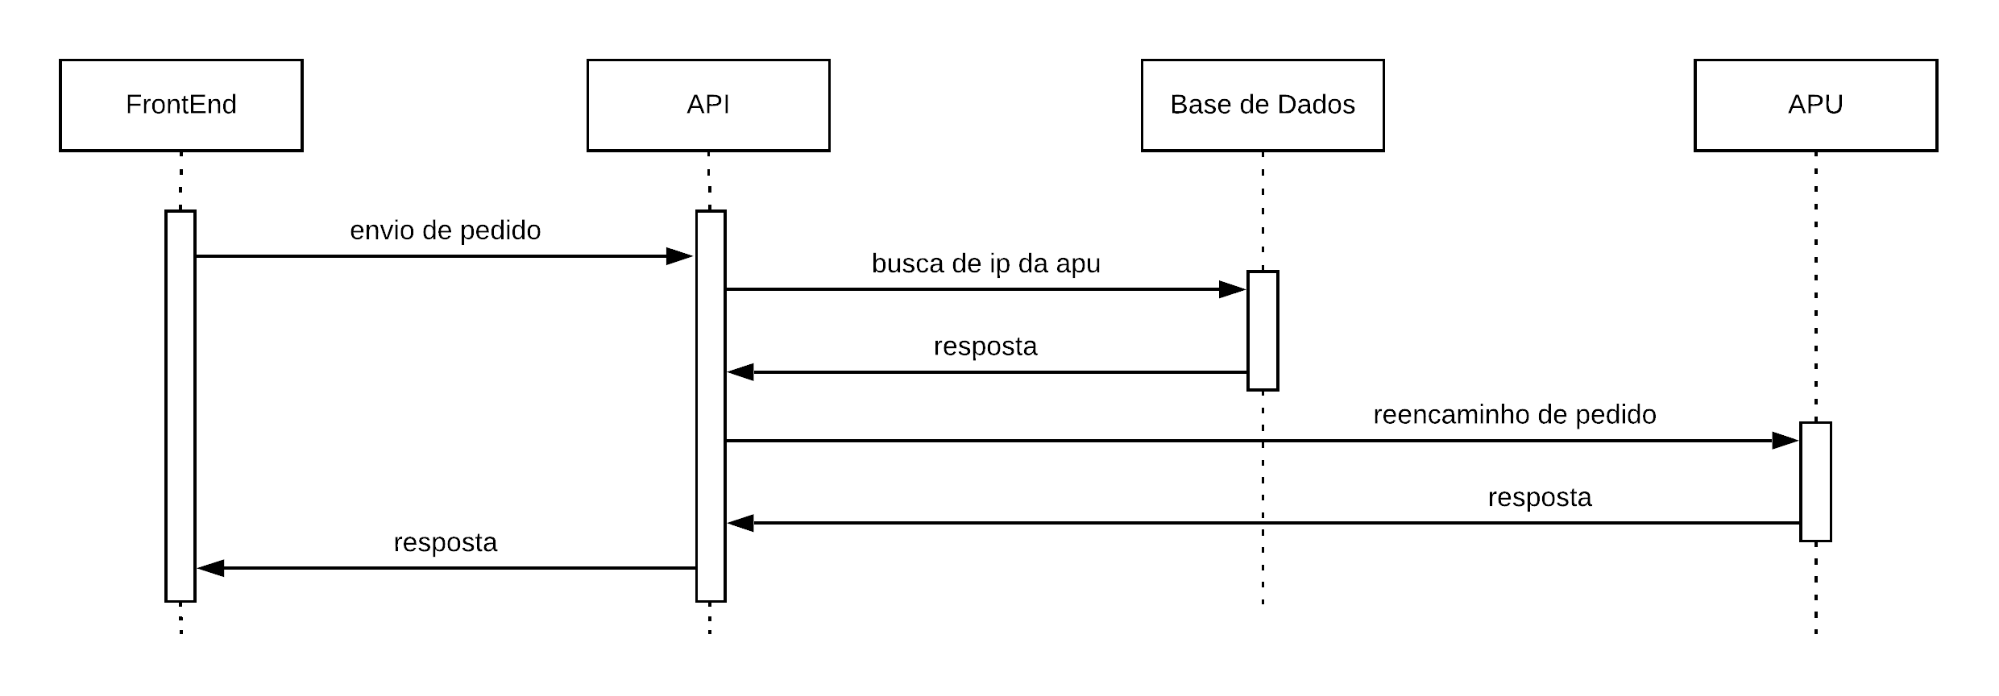
\includegraphics[width=0.8\textwidth]{images/fluxo3.png}
    \caption{Fluxo de comunicação Proxy, para os métodos GET, POST e PUT}
    \label{fig:proxy}
\end{figure}
\newpage
Um dos objetivos expectáveis ao agendar uma experiência, é que esta se possa iniciar de forma automática, sem a necessidade da presença do utilizador que deseja realizar a experiência ou de um administrador. Deste modo, esta pode acontecer mesmo em horários não convencionais, uma vez que não existe a necessidade de presença e/ou de disponibilidade para observar o decorrer da experiência.\newline\\
Uma vez lançada, a API ficará constantemente, em segundo plano, a pesquisar pela próxima experiência que deve ser executada. Posteriormente, com recurso à interface APScheduler, a API irá iniciar esta experiência no instante temporal agendado. Para que este início automático se dê, as configurações das APUs são enviadas individualmente para cada APU envolvida na experiência e esta irá retornar sobre o seu estado. Isto é, irá indicar se a mesma foi ou não iniciada. Para além disso, esta informação é atualizada na base de dados de forma a ficar registada. Uma vez terminada a experiência, o servidor consulta todas as APUs envolvidas no processo de forma a validar a realização da experiência. Após isso, estas informações são guardadas na base de dados. Após o armazenamento das informações, o servidor notifica, via email, o utilizador que agendou a experiência sobre o estado e resultados da experiência, utilizando o Flask-Mail.
\begin{figure}[!ht]
    \centering
    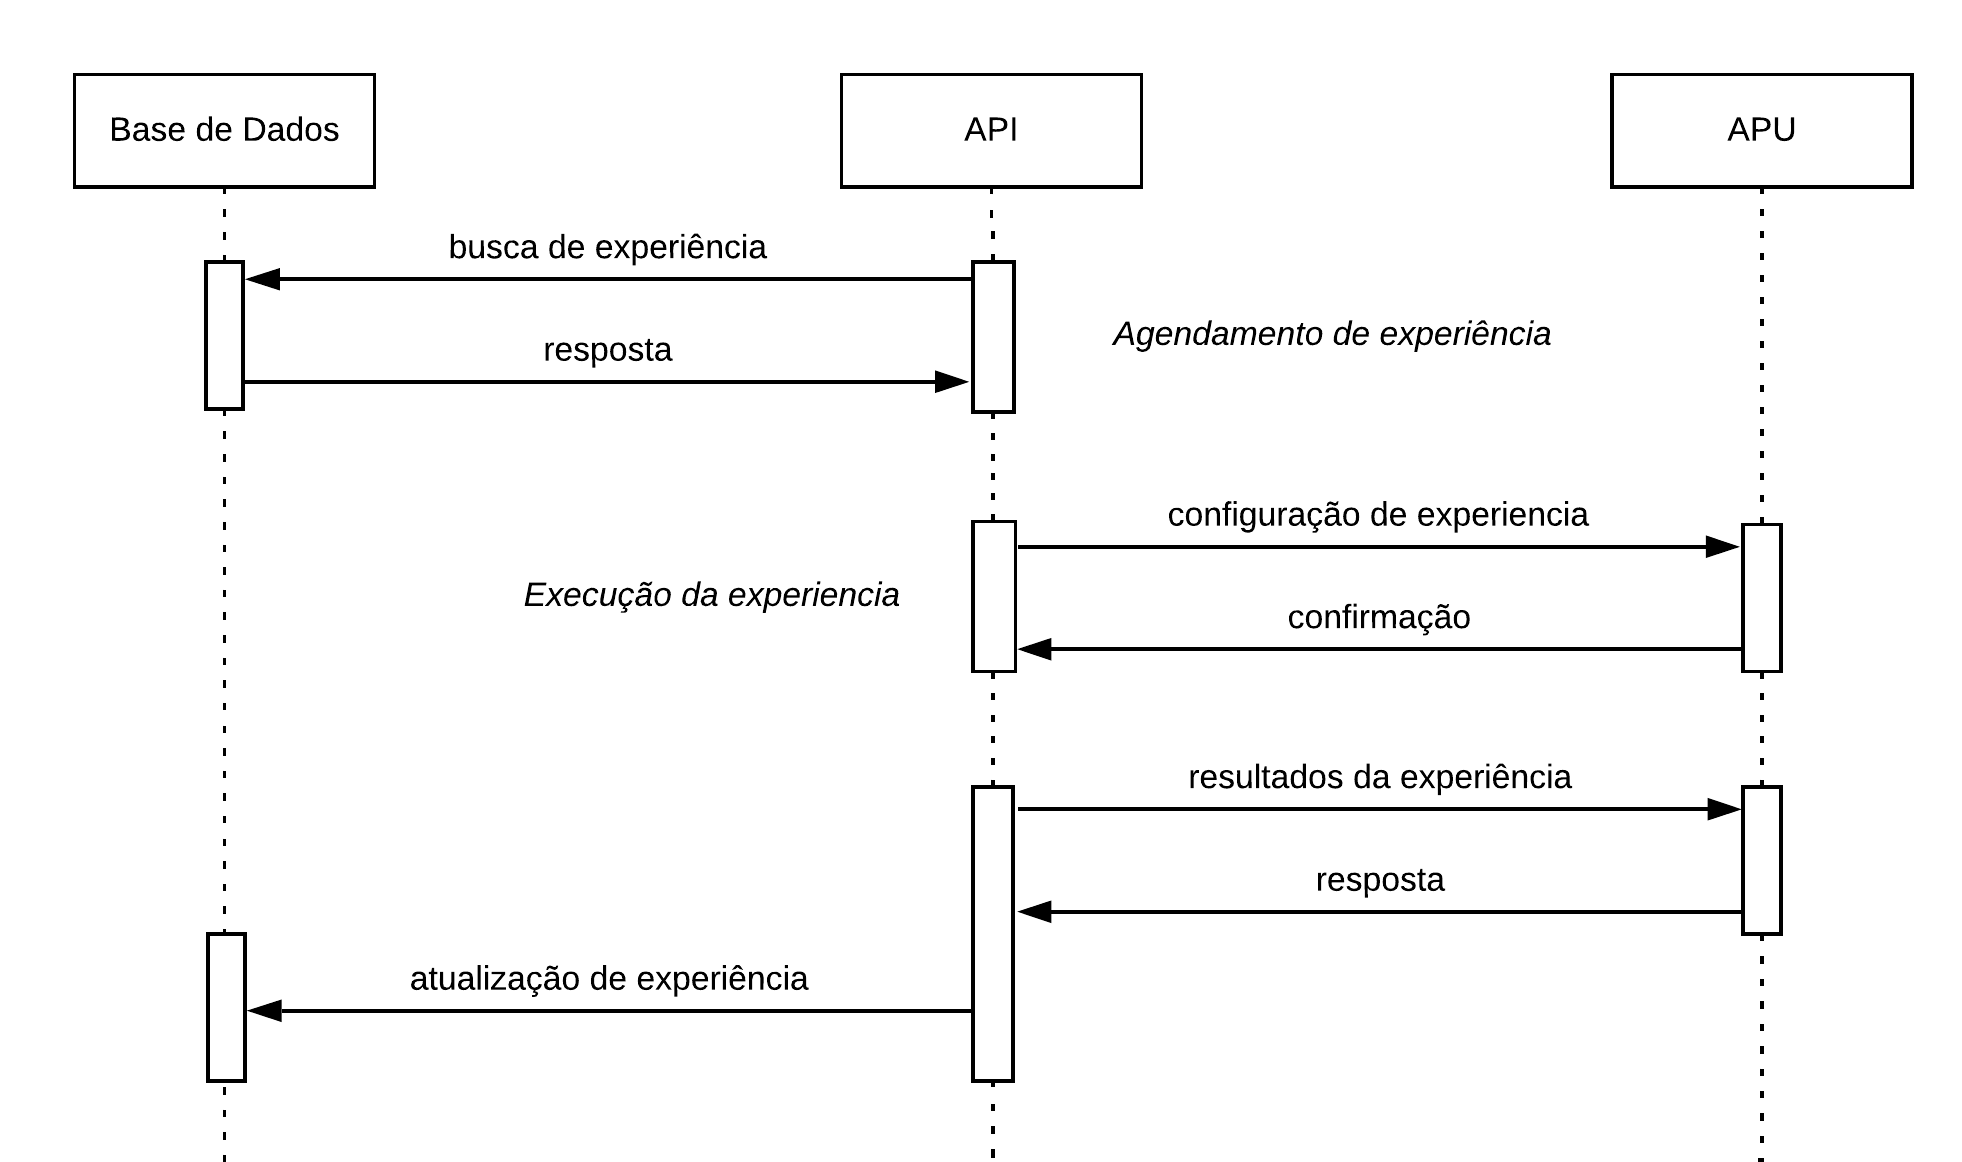
\includegraphics[width=0.9\textwidth]{images/fluxo4.png}
    \caption{Fluxo de comunicação Proxy, para os métodos GET e POST}
    \label{fig:agendamento}
\end{figure}
\subsection{Testes}
De forma a garantir que o desenvolvimento de novas funcionalidades não afete o comportamento das que já estão estabelecidas, foram realizados diversos testes para garantir a integridade do código.\newline\\
Os testes de integração foram criados utilizando a framework Pytest em conjunto com uma base de dados em memória, criada com recurso ao SQLite. Estes foram realizados em todas os caminhos disponibilizados pela API, excluindo apenas os caminhos que comunicam com as APUS, uma vez que eles constituem proxys. Como tal, estes não necessitam de ser testados, visto que simplesmente redirecionam a informação recebida para o APU de destino, sem que exista qualquer tipo de tratamento.\newline\\
A percentagem de cobertura prevista foi de 90\% do código do módulo views. Esta métrica foi definida de forma a ser aprovada nos padrões de qualidade do sonarqube \cite{sonar} e medida através de ferramentas próprias do Pytest.

\section{Camada de visualização}
O Frontend, tal como mencionado anteriormente, foi implementado com recurso a Django. Para esta implementação, a abordagem tradicional típica desta framework (consumo direto dos dados existentes na base de dados) foi colocada de parte e optou-se pelo consumo de dados através de uma API Rest. É de salientar que, apesar desta mudança de abordagem, a gestão de utilizadores e autenticação dos mesmos faz jus às ferramentas disponibilizadas por esta framework.\newline
O modelo de consumo direto de dados, como foi mencionado, deu lugar a pedidos REST. Assim, em todas as páginas existe uma troca de pedidos entre o servidor Django e a API Flask, de modo a que estas possam ser renderizadas. Podemos assim considerar, que para renderizar uma vista web do frontend ocorre o seguinte procedimento:
\begin{enumerate}[noitemsep]
    \item Chamada do path da API correspondente à vista que queremos renderizar através do verbo rest correspondente;
    \item Validação do resultado e consequente status code:
    \SubItem {Caso o status code não seja o expectável é retornado uma página de erro informando o utilizador acerca do erro ocorrido;}
    \SubItem{Caso não haja nenhum problema, a vista web é renderizada com a informação obtida.}
\end{enumerate}

\subsection{Autenticação}
Toda a plataforma requer autorizações para ser acedida. Isto é, para os utilizadores interagirem com a mesma, têm que estar, obrigatoriamente, com o seu login efetuado. Caso o utilizador pretenda aceder a uma página quando não está com o seu login efetuado é automaticamente redirecionado para a página de login.\newline
É importante realçar que esta implementação da autenticação recorre ao modelo de autenticação já existente na framework Django.\hfill\break
\begin{figure}[!ht]
    \centering
    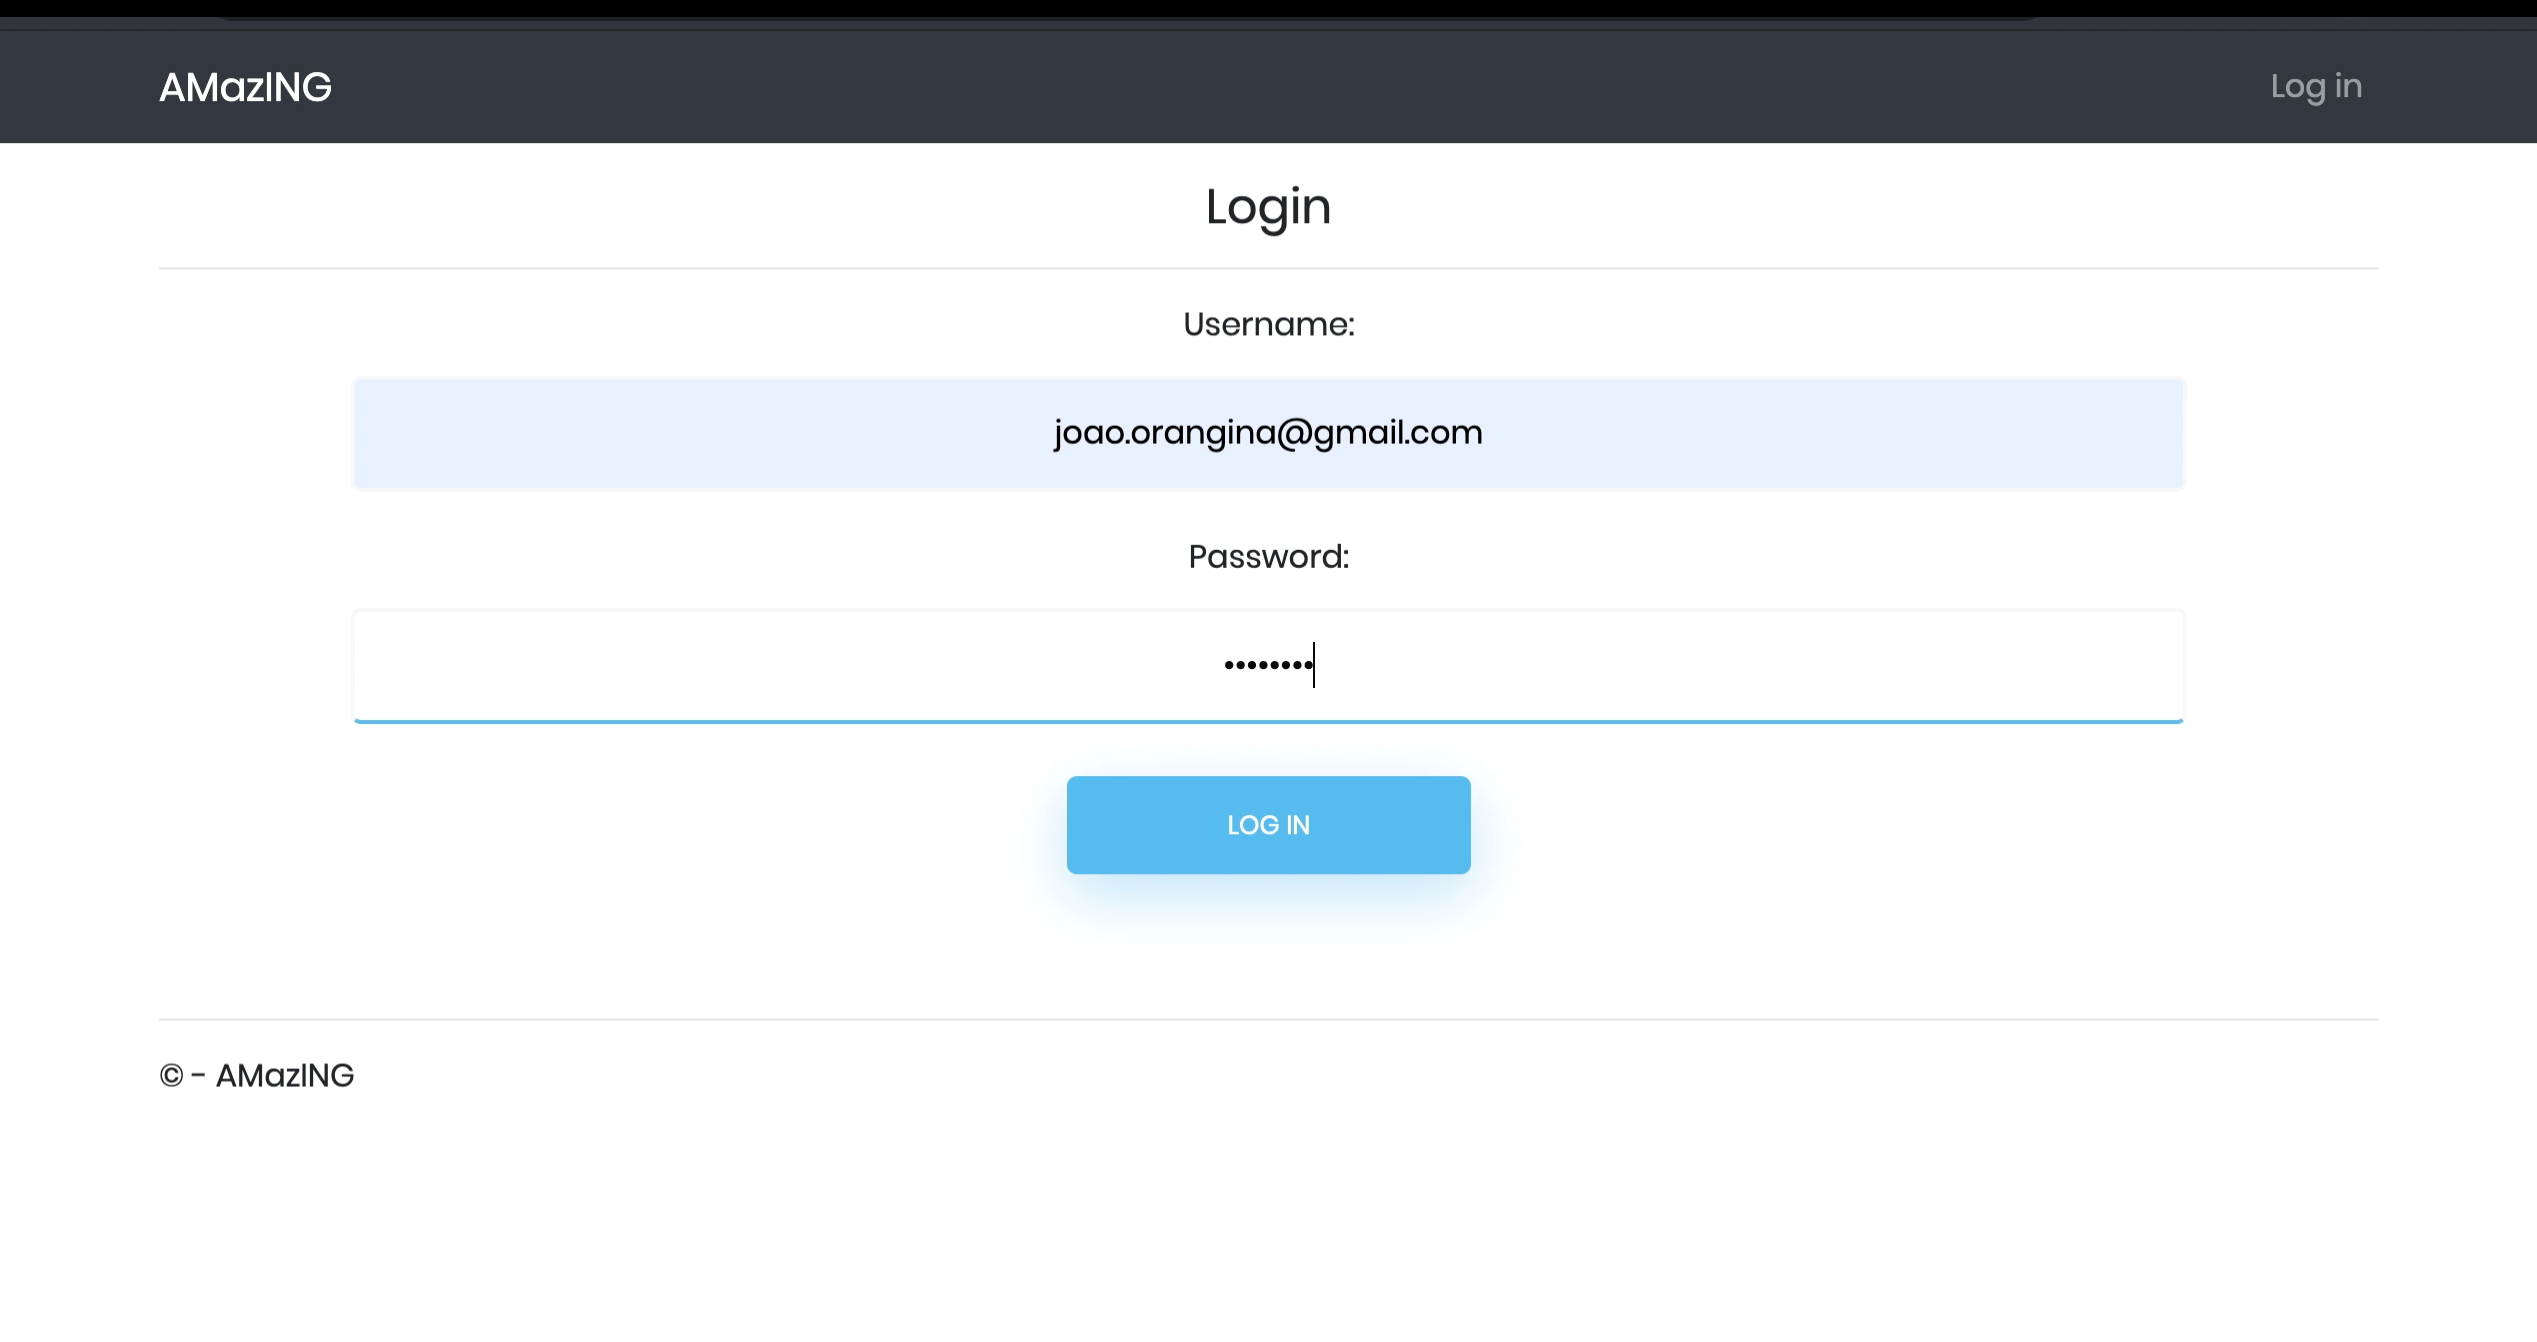
\includegraphics[width=0.9\textwidth]{images/login.png}
    \caption{Autenticação - Frontend}
    \label{fig:login}
\end{figure}
\newpage
\subsection{Estado da rede AMazING}
Assim que o utilizador efetua o seu login, é redirecionado para uma página em que encontra a informação relativa à rede AMazING. Assim sendo, pode consultar a disposição gráfica dos nós no edifício do IT bem como o seu estado (on e off). O estado é obtido através de um pedido http à API Flask.
\begin{figure}[!ht]
    \centering
    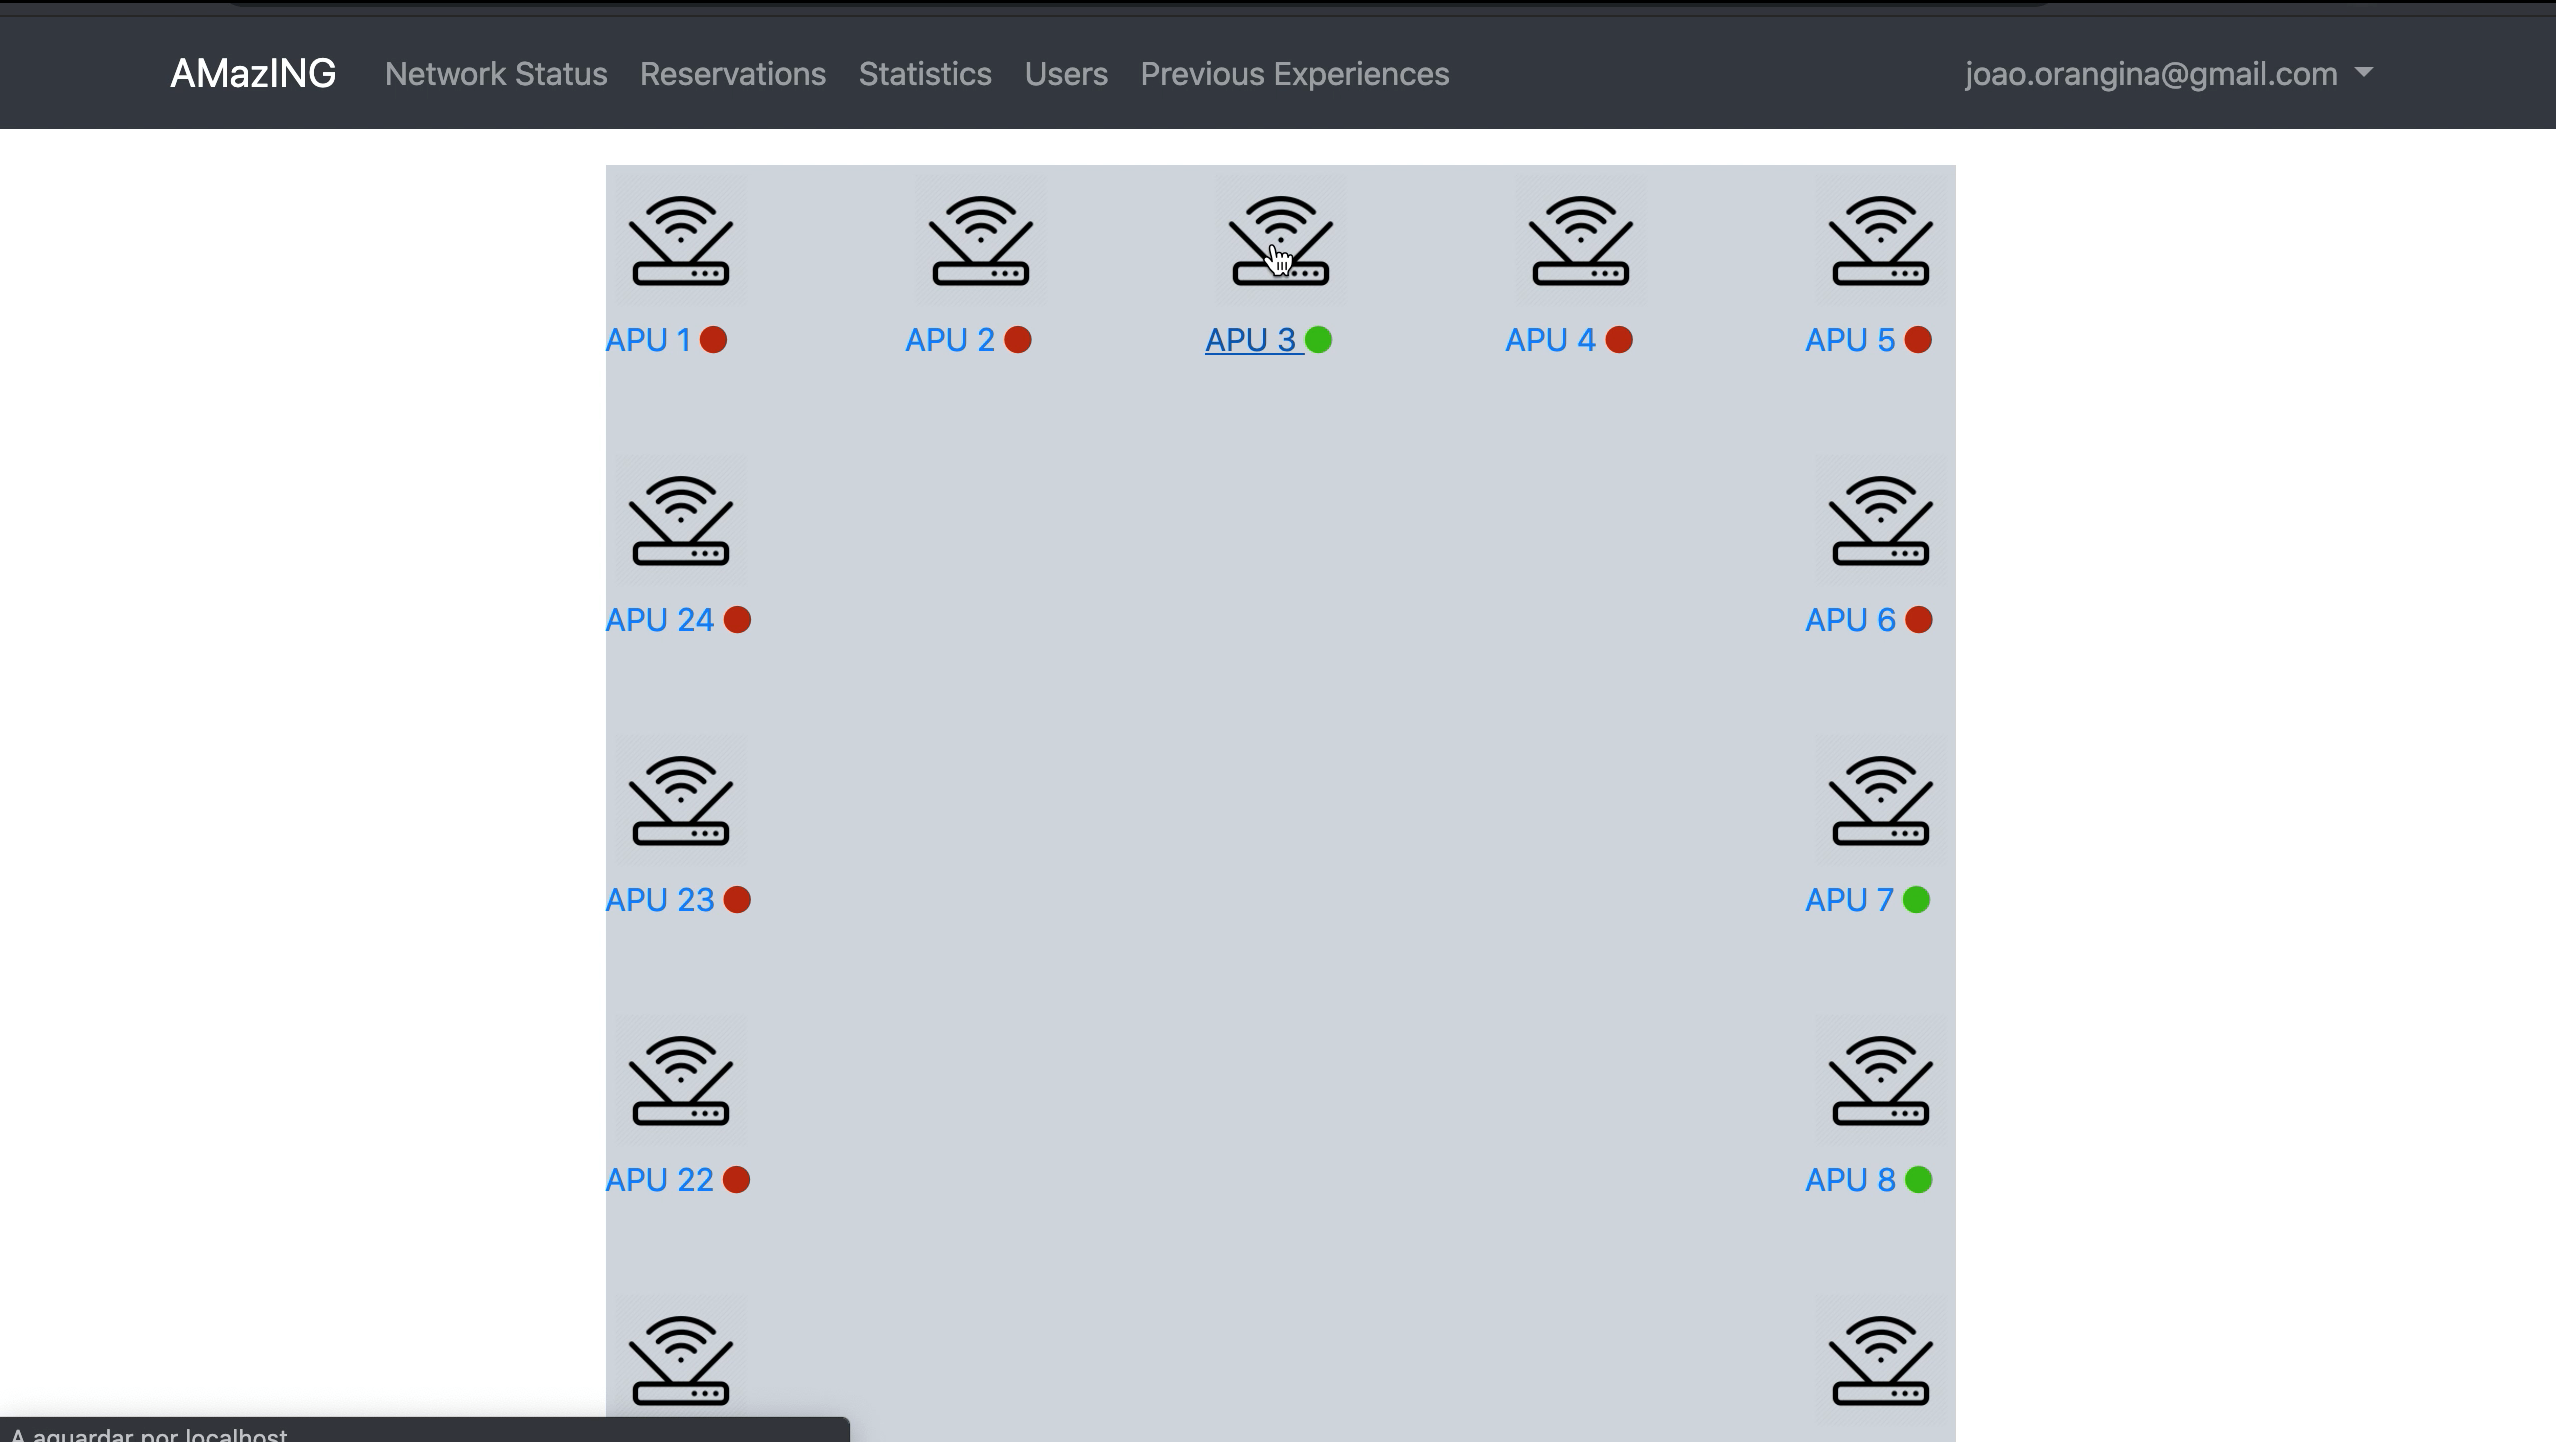
\includegraphics[width=0.9\textwidth]{images/main_page.png}
    \caption{Disposição e estado das APUs}
    \label{fig:mainpage}
\end{figure}

\subsection{Informação de um APU}
Apesar de se ter uma vista geral dos APUs, é possível ter, também, uma vista individual sobre cada APU. Isto é, é possível interagir de forma individual com cada um dos nós. Quando se consulta um APU, é apresenta a informação relativa às interfaces que estão ligadas e/ou desligadas, sendo possível interagir com ambas.
A obtenção desta informação é feita com recurso a uma chamada à API Flask via HTTP Request:
\begin{lstlisting}[language=python,caption={Pedido de informação de um APU},breaklines=true,label={code:apuinfo}]

def processNode(request, nodeID, content=None, iName=None):
    if request.user.is_authenticated:
        token = tokenizer.nodeToken(request.user.email)
        r = requests.get(API + "node/" + str(nodeID), headers={'Authorization': 'Bearer ' + token})
        if r.status_code != 200:
            return HttpResponseRedirect(request.META.get('HTTP_REFERER', '/'))
        json = r.json()
        token = tokenizer.gerateEmailToken(request.user.email)
        r = requests.get(API + "profile", headers={'Authorization': 'Bearer ' + token})
        if r.status_code != 200:
            return HttpResponseRedirect(request.META.get('HTTP_REFERER', '/'))
        role = r.json()
        token = tokenizer.nodeToken(request.user.email)
        r = requests.get(API + "experience/now", headers={'Authorization': 'Bearer ' + token})
        if r.status_code != 200:
            return HttpResponseRedirect(request.META.get('HTTP_REFERER', '/'))
\end{lstlisting}
\hfill\break
É de notar que são executados três pedidos HTTP à API uma vez que é necessário obter várias informações. Resumidamente, é necessário ir buscar as informações respetivas do nó (primeiro pedido), ir buscar as informações de acesso do utilizador que faz o pedido, uma vez que diferentes tipos de utilizadores têm direito a diferentes tipos de acessos junto destes nós e, por último, informação sobre experiências de modo a que, caso esteja a decorrer uma experiência que não pertença ao utilizador que efetua o pedido, ele não possa interagir com os APUs. Caso não esteja a ocorrer uma experiência, de modo a conseguir interagir com os APUs, terá que fazer um registo de uma experiência.\hfill\break
\newpage
\begin{figure}[!ht]
    \centering
    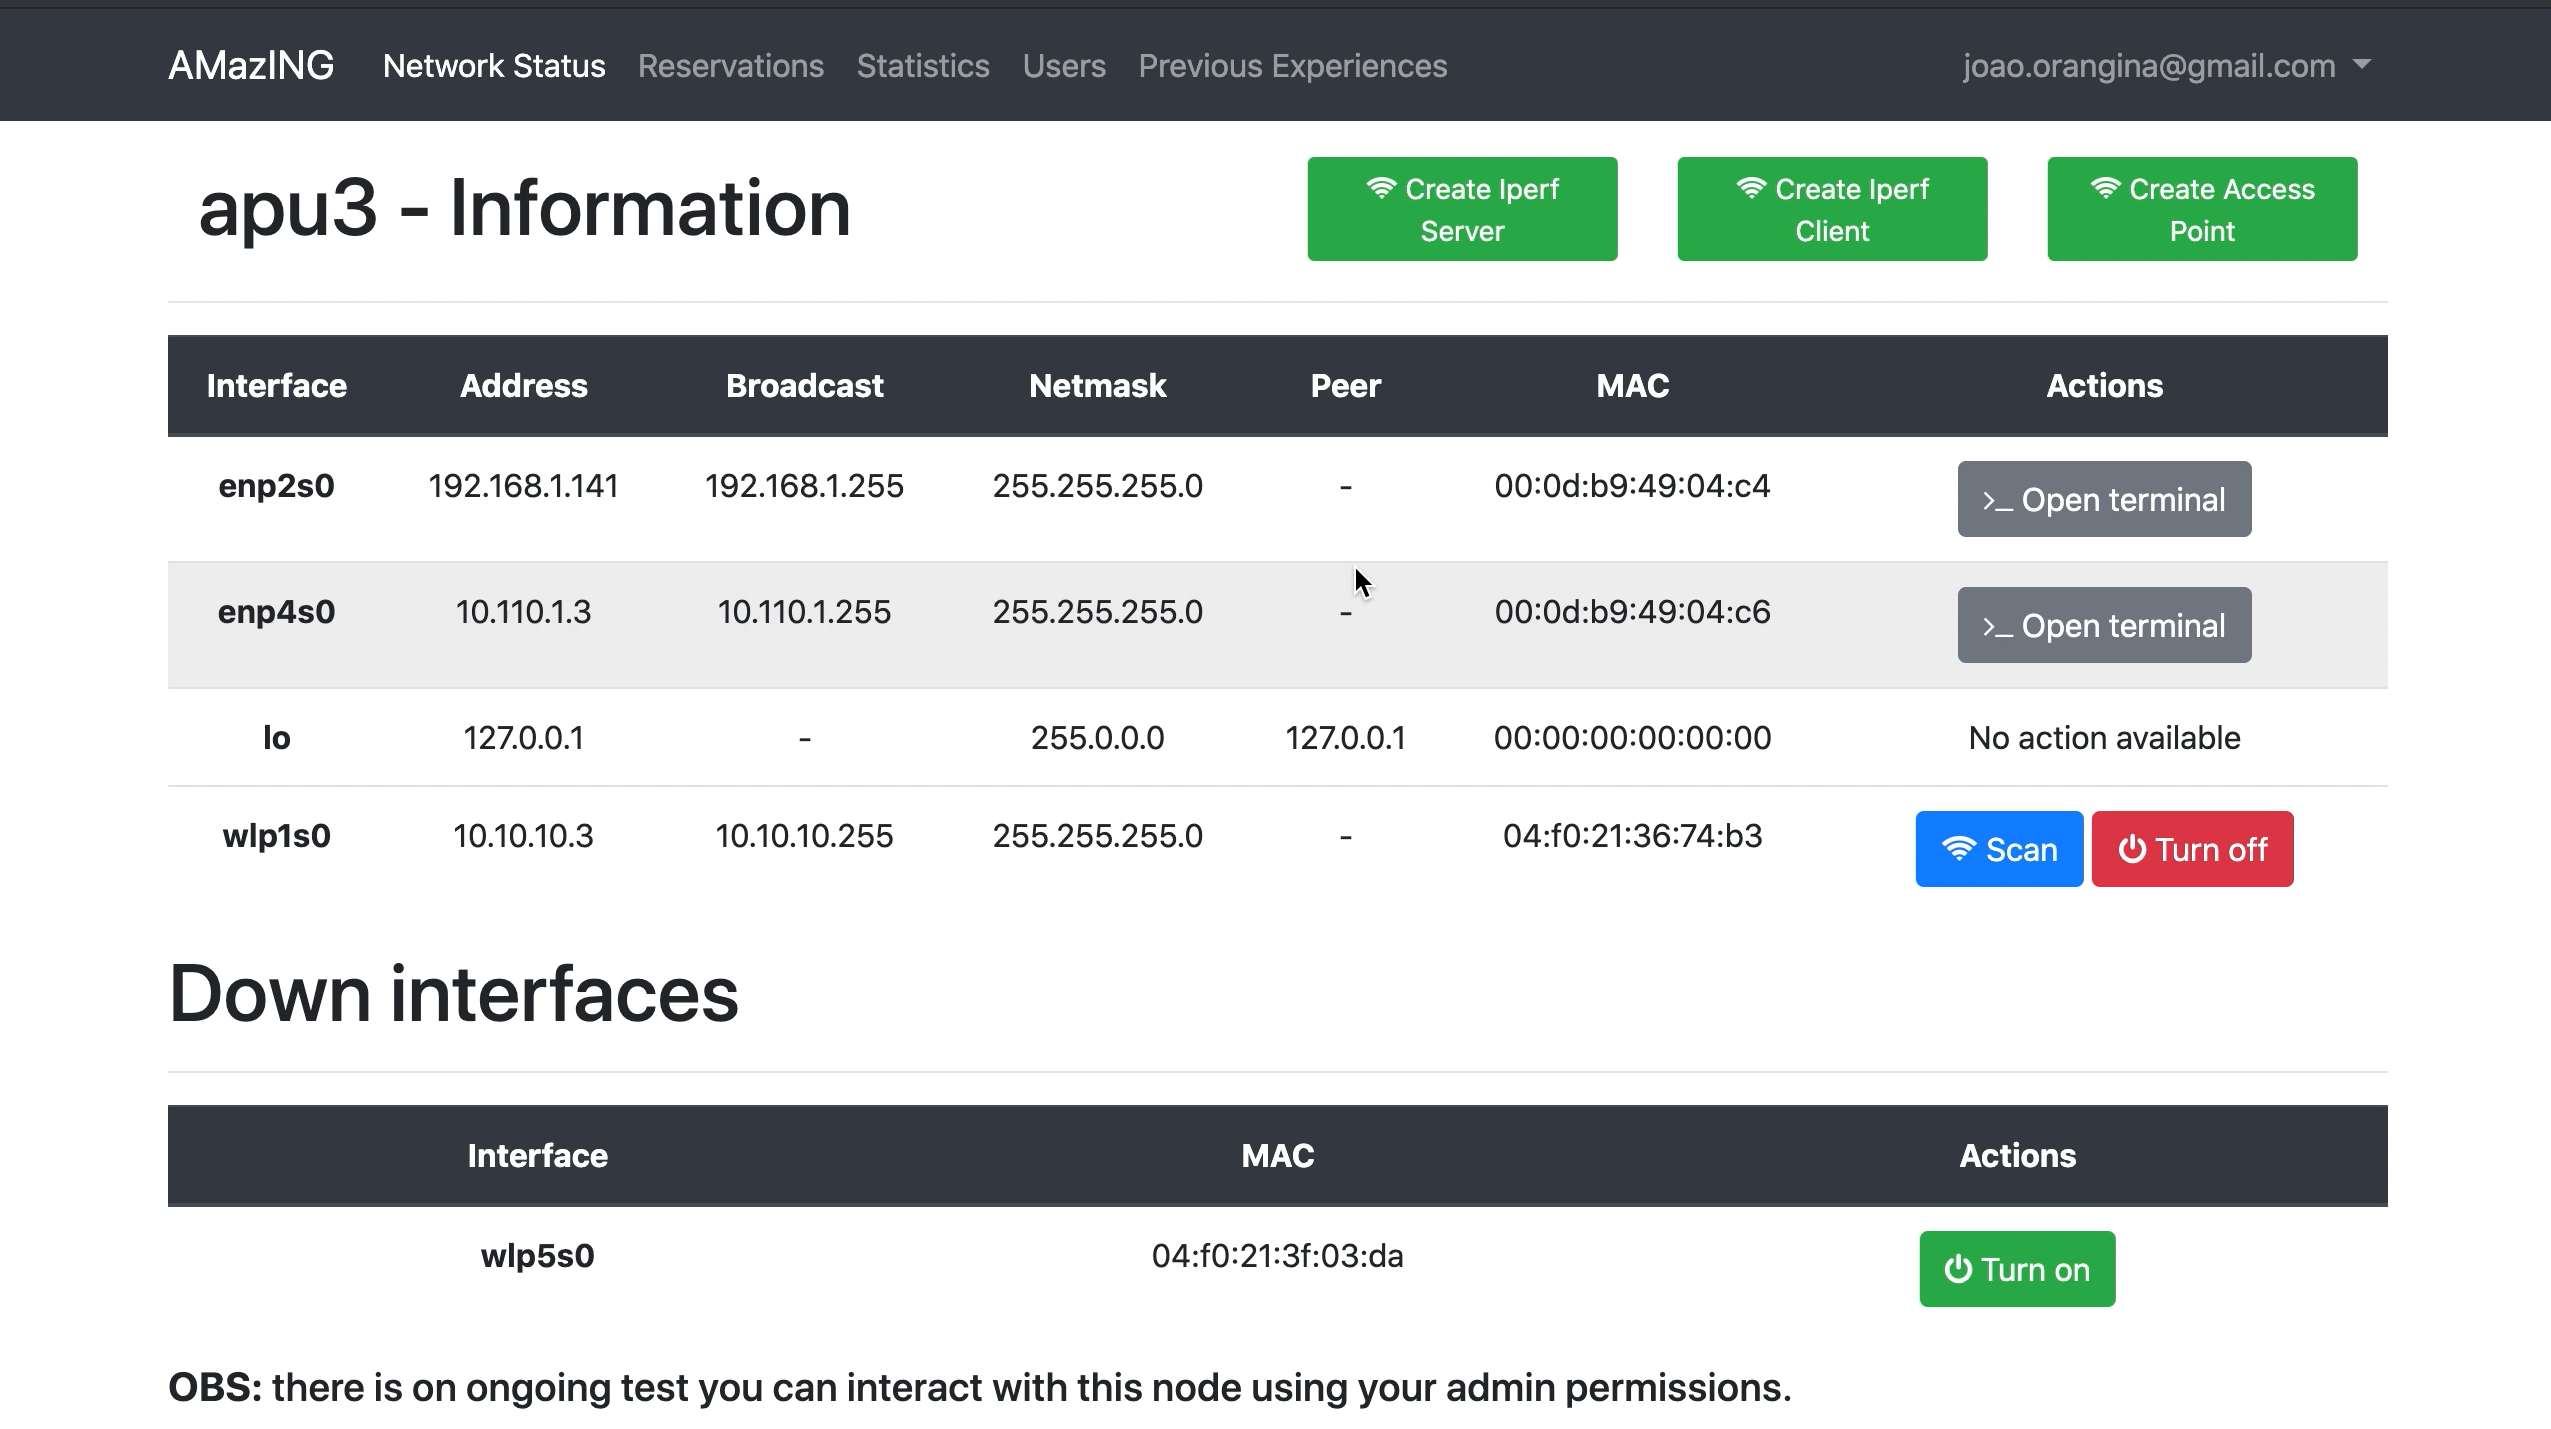
\includegraphics[width=0.9\textwidth]{images/node_stats.png}
    \caption{Informação de um Nó}
    \label{fig:nodeinfo}
\end{figure}

\subsection{Templates}
Tal como mencionado anteriormente, os utilizadores menos experientes não têm acesso ao terminal. Como tal, são disponibilizados templates pré-definidos, nos quais apenas precisam de preencher os campos. Após isso, o APU é configurado automaticamente.

\subsubsection{Criação de um AP}
Acedendo a um APU específico, o utilizador dispõe de um botão que lhe permite criar um Access Point de forma simples e intuitiva, tendo apenas de preencher os campos que lhe são pedidos:\hfill\break
\newpage
\begin{figure}[!ht]
    \centering
    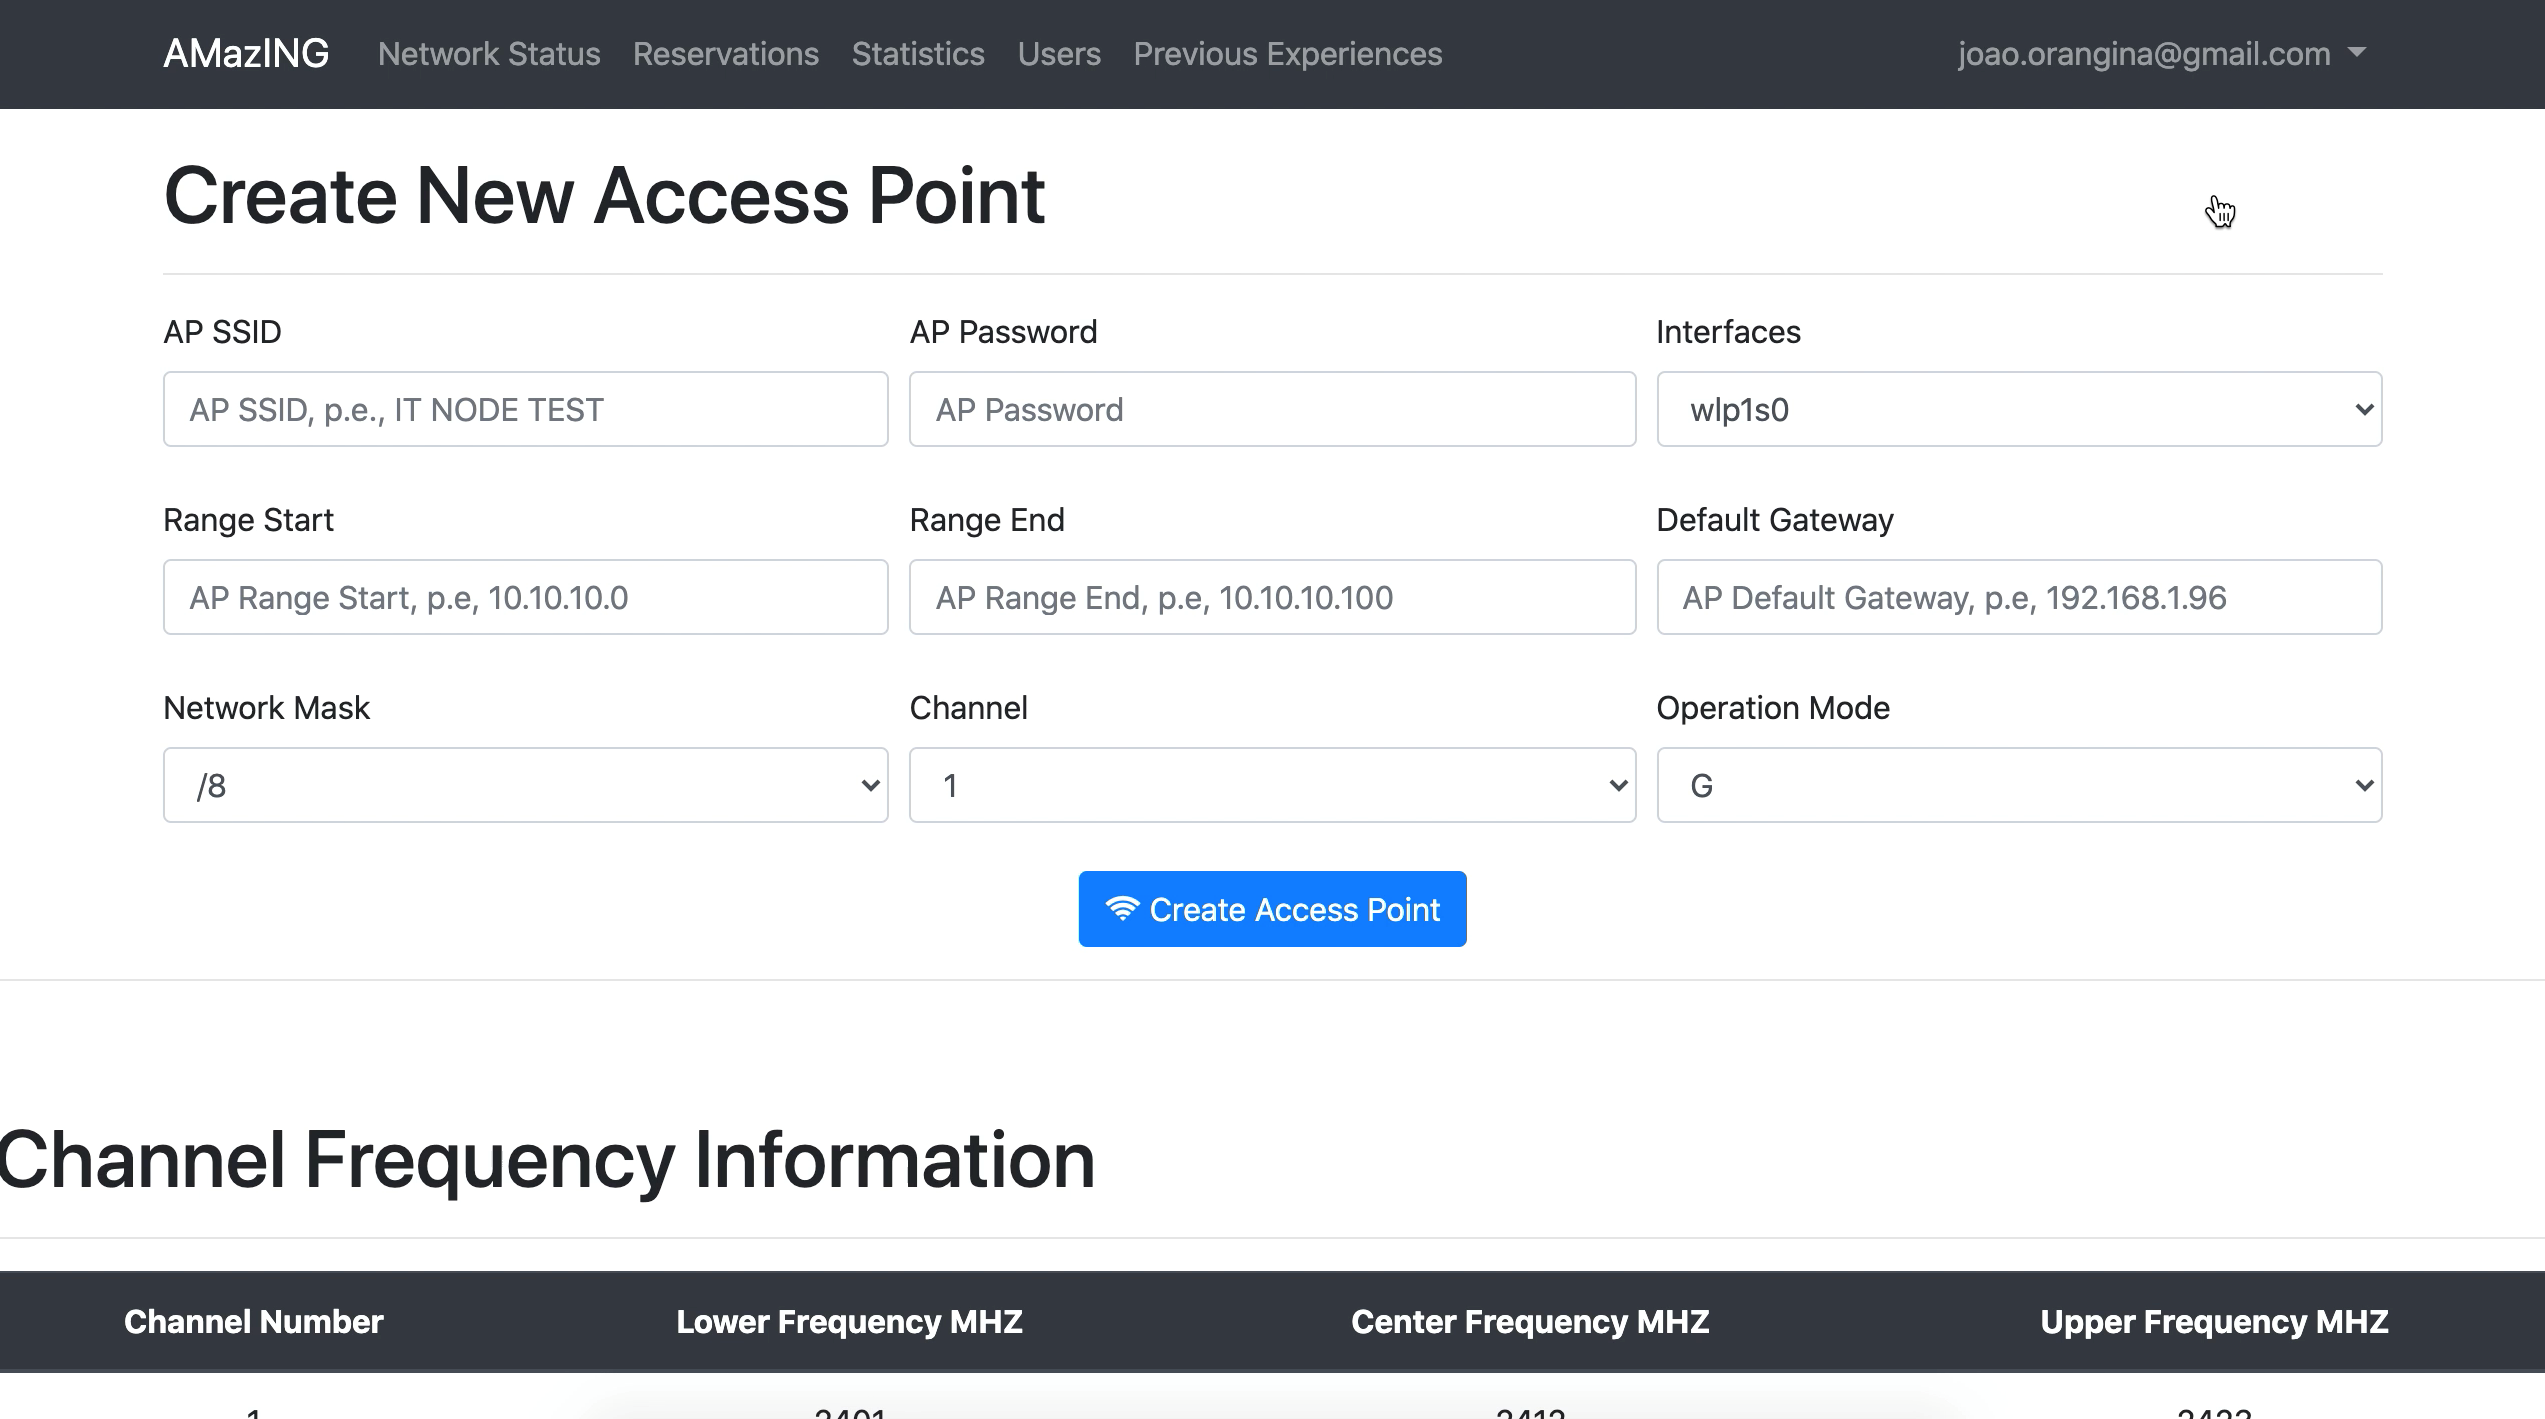
\includegraphics[width=0.9\textwidth]{images/create_ap.png}
    \caption{Criação de um AP}
    \label{fig:createap}
\end{figure}
\hfill\break
Preenchendo estes campos, e sendo todos eles válidos, é executado um pedido HTTP à API por forma a que este seja redirecionado para o APU com o qual se pretende comunicar.
\begin{lstlisting}[language=python,caption={Criação de um AP},breaklines=true,label={code:createap}]
msg = {
    'APSSID': APSSID.replace(" ", "-"),
    'APPW': APPW, 'Channel': Channel,
    'RangeStart': RangeStart, 'RangeEnd': RangeEnd,
    'hw_mode': hw_mode, 'DFGateway': DFGateway,
    'Netmask': Netmask, 'interface': interface
}
r = requests.post(API + "node/" + str(nodeID) + "/accesspoint", json=msg,
                  headers={'Authorization': 'Bearer ' + token})
\end{lstlisting}
Após este pedido ser efetuado é aguardada uma resposta. Após isso, o utilizador é informado sobre o resultado da ação que acabou de efetuar. Em caso de sucesso, é enviada uma mensagem de sucesso. No caso de ocorrer um erro, é enviada uma mensagem de erro genérica e é armazenada a informação do erro num logger próprio para o efeito.
\begin{lstlisting}[language=python,caption={Resultado da comunicação Frontend - APU},breaklines=true,label={code:createap}]
if r.status_code != 200:
    logger.info(str(r.status_code) + str(r.text))
    messages.error(request, json['msg'])
    return redirect('nodestatus', nodeID=nodeID)

messages.info(request, json['msg'])
return processNode(request=request, nodeID=nodeID)
\end{lstlisting}

\subsection{Criação de um Iperf Client}
À semelhança do que acontece no AP, existe a possibilidade de criar um Iperf Client através de um template, necessitando apenas de preencher as informações pedidas por este. A forma como é tratado é similar ao AP, existindo na mesma validação de informação. Após a validação, a informação é enviada para a API que a irá redirecionar para a APU correspondente.
\begin{figure}[!ht]
    \centering
    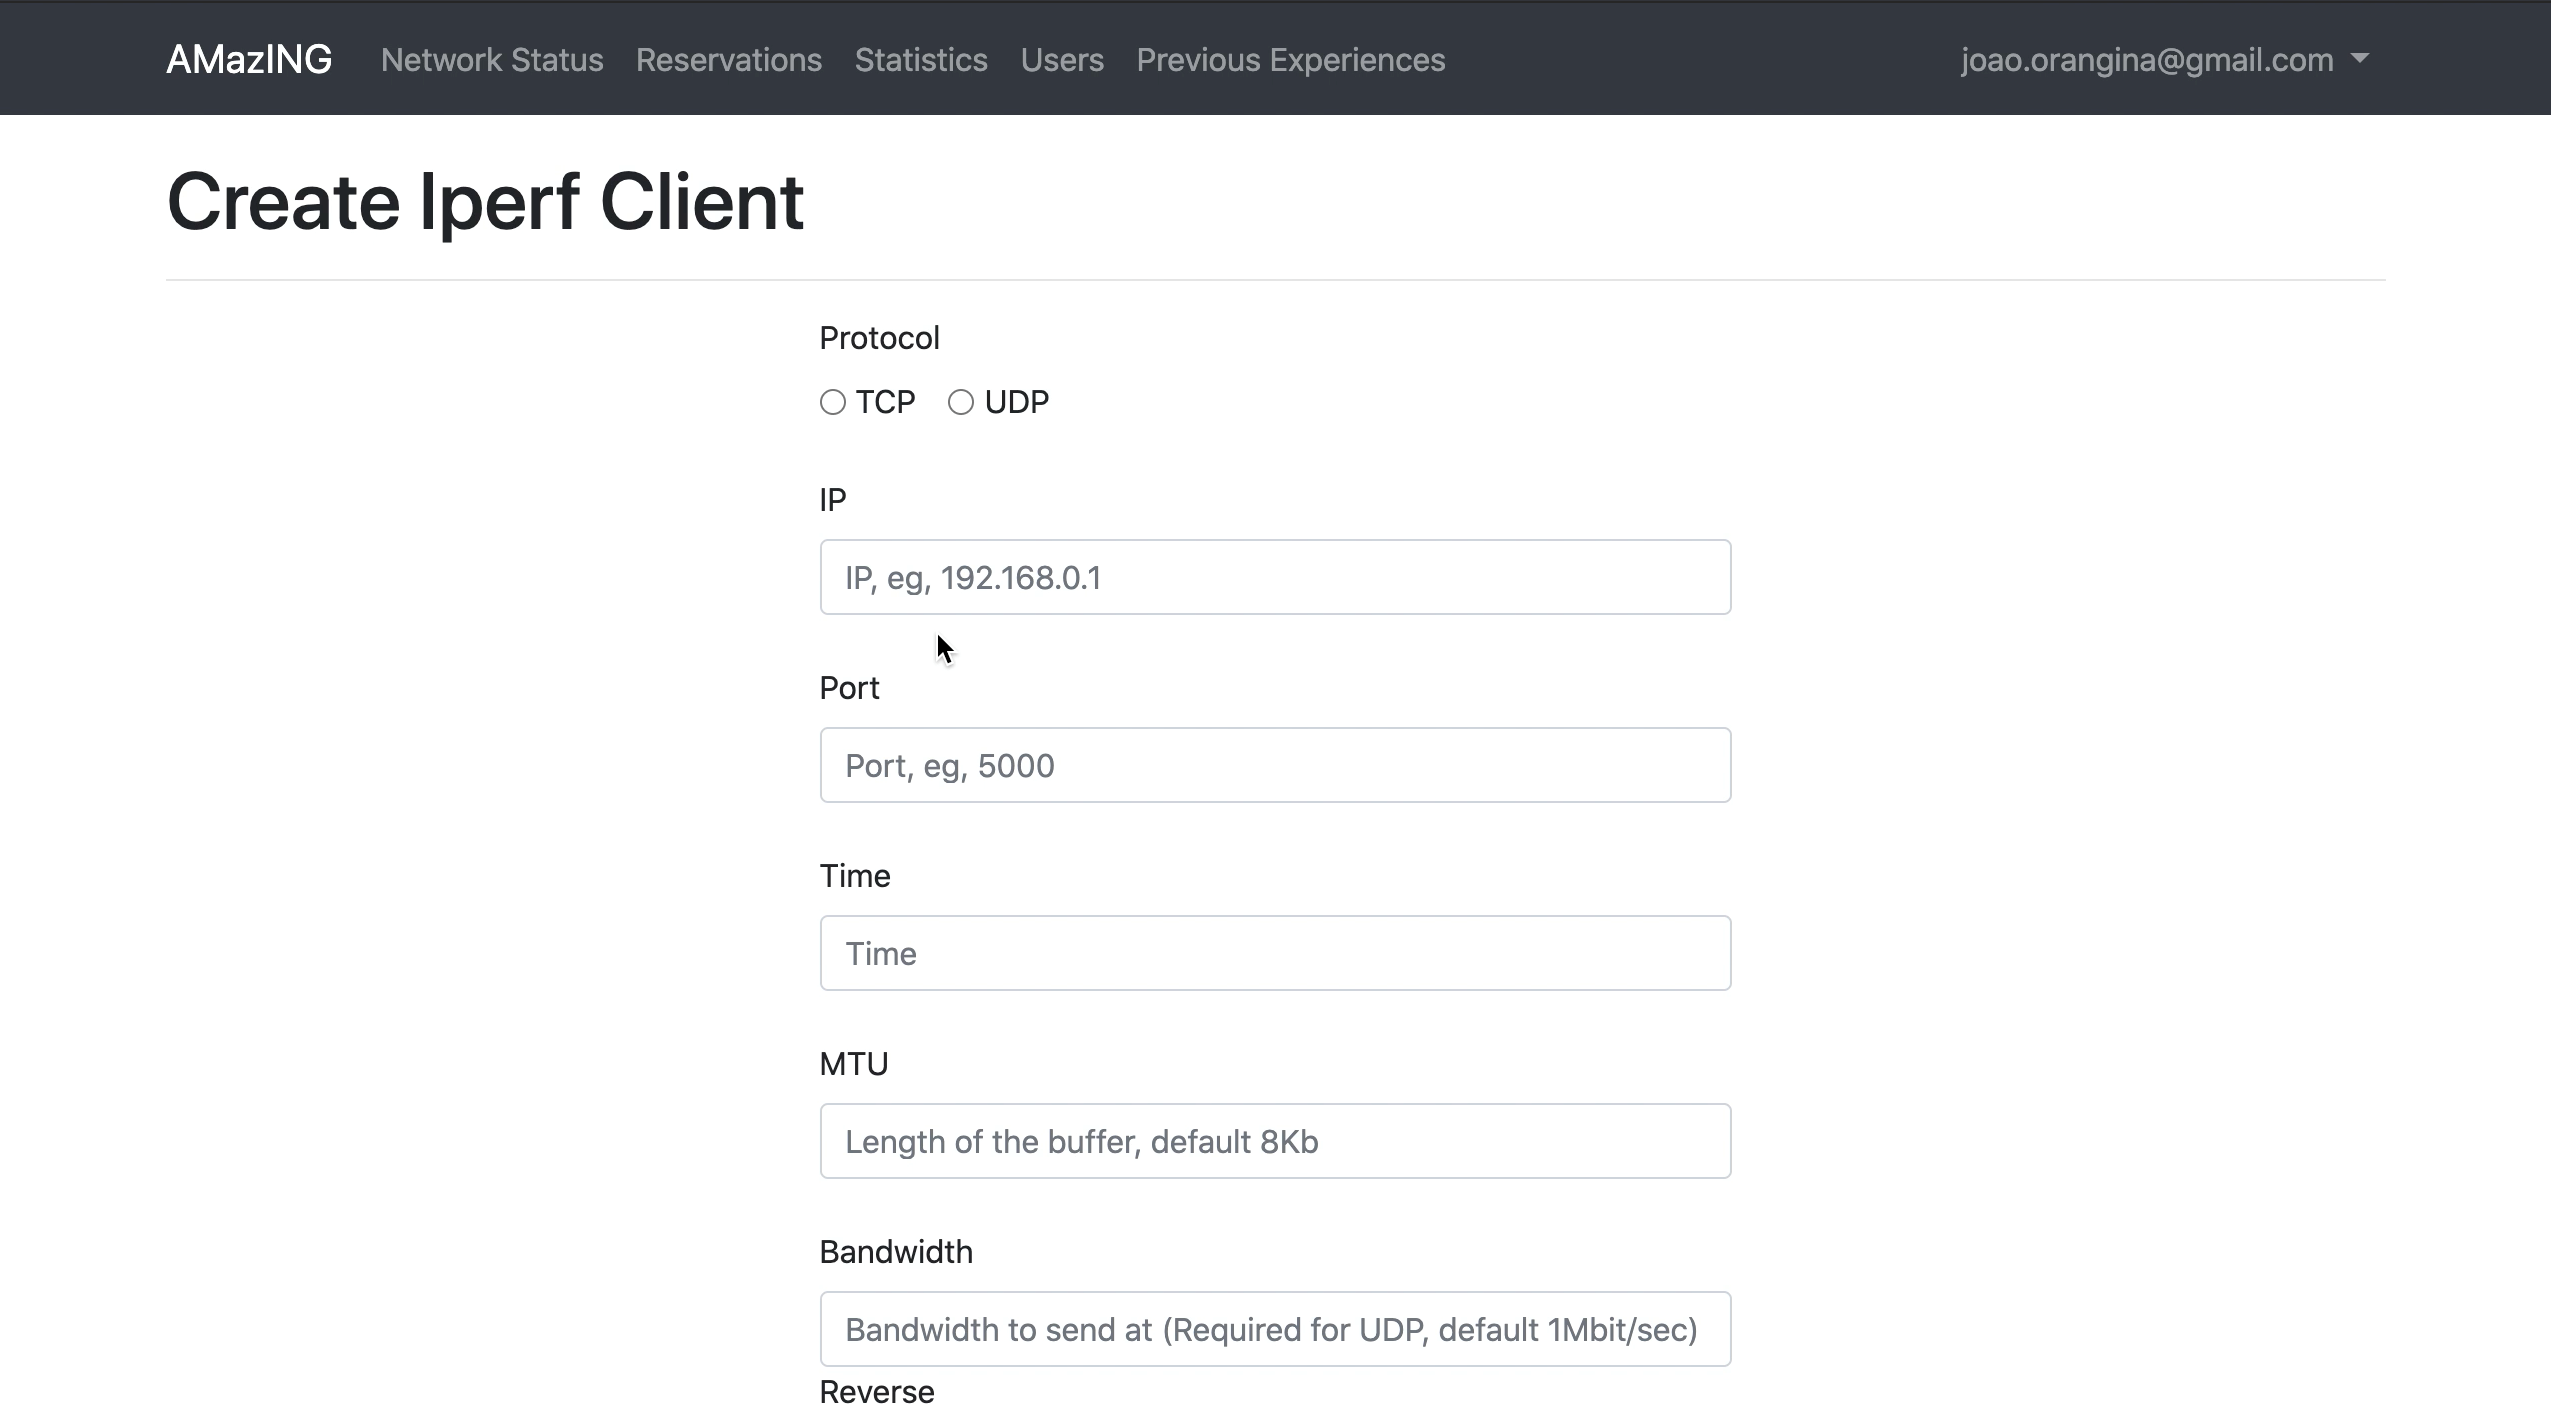
\includegraphics[width=0.7\textwidth]{images/create_iperfcli.png}
    \caption{Exemplo de criação de um Iperf Client}
    \label{fig:iperfcli}
\end{figure}

\subsection{Criação de um Iperf Server}
Tal como no caso do Iperf Client, é possível criar um Iperf Server recorrendo apenas ao template existente e preenchendo os campos que este necessita.
\begin{figure}[!ht]
    \centering
    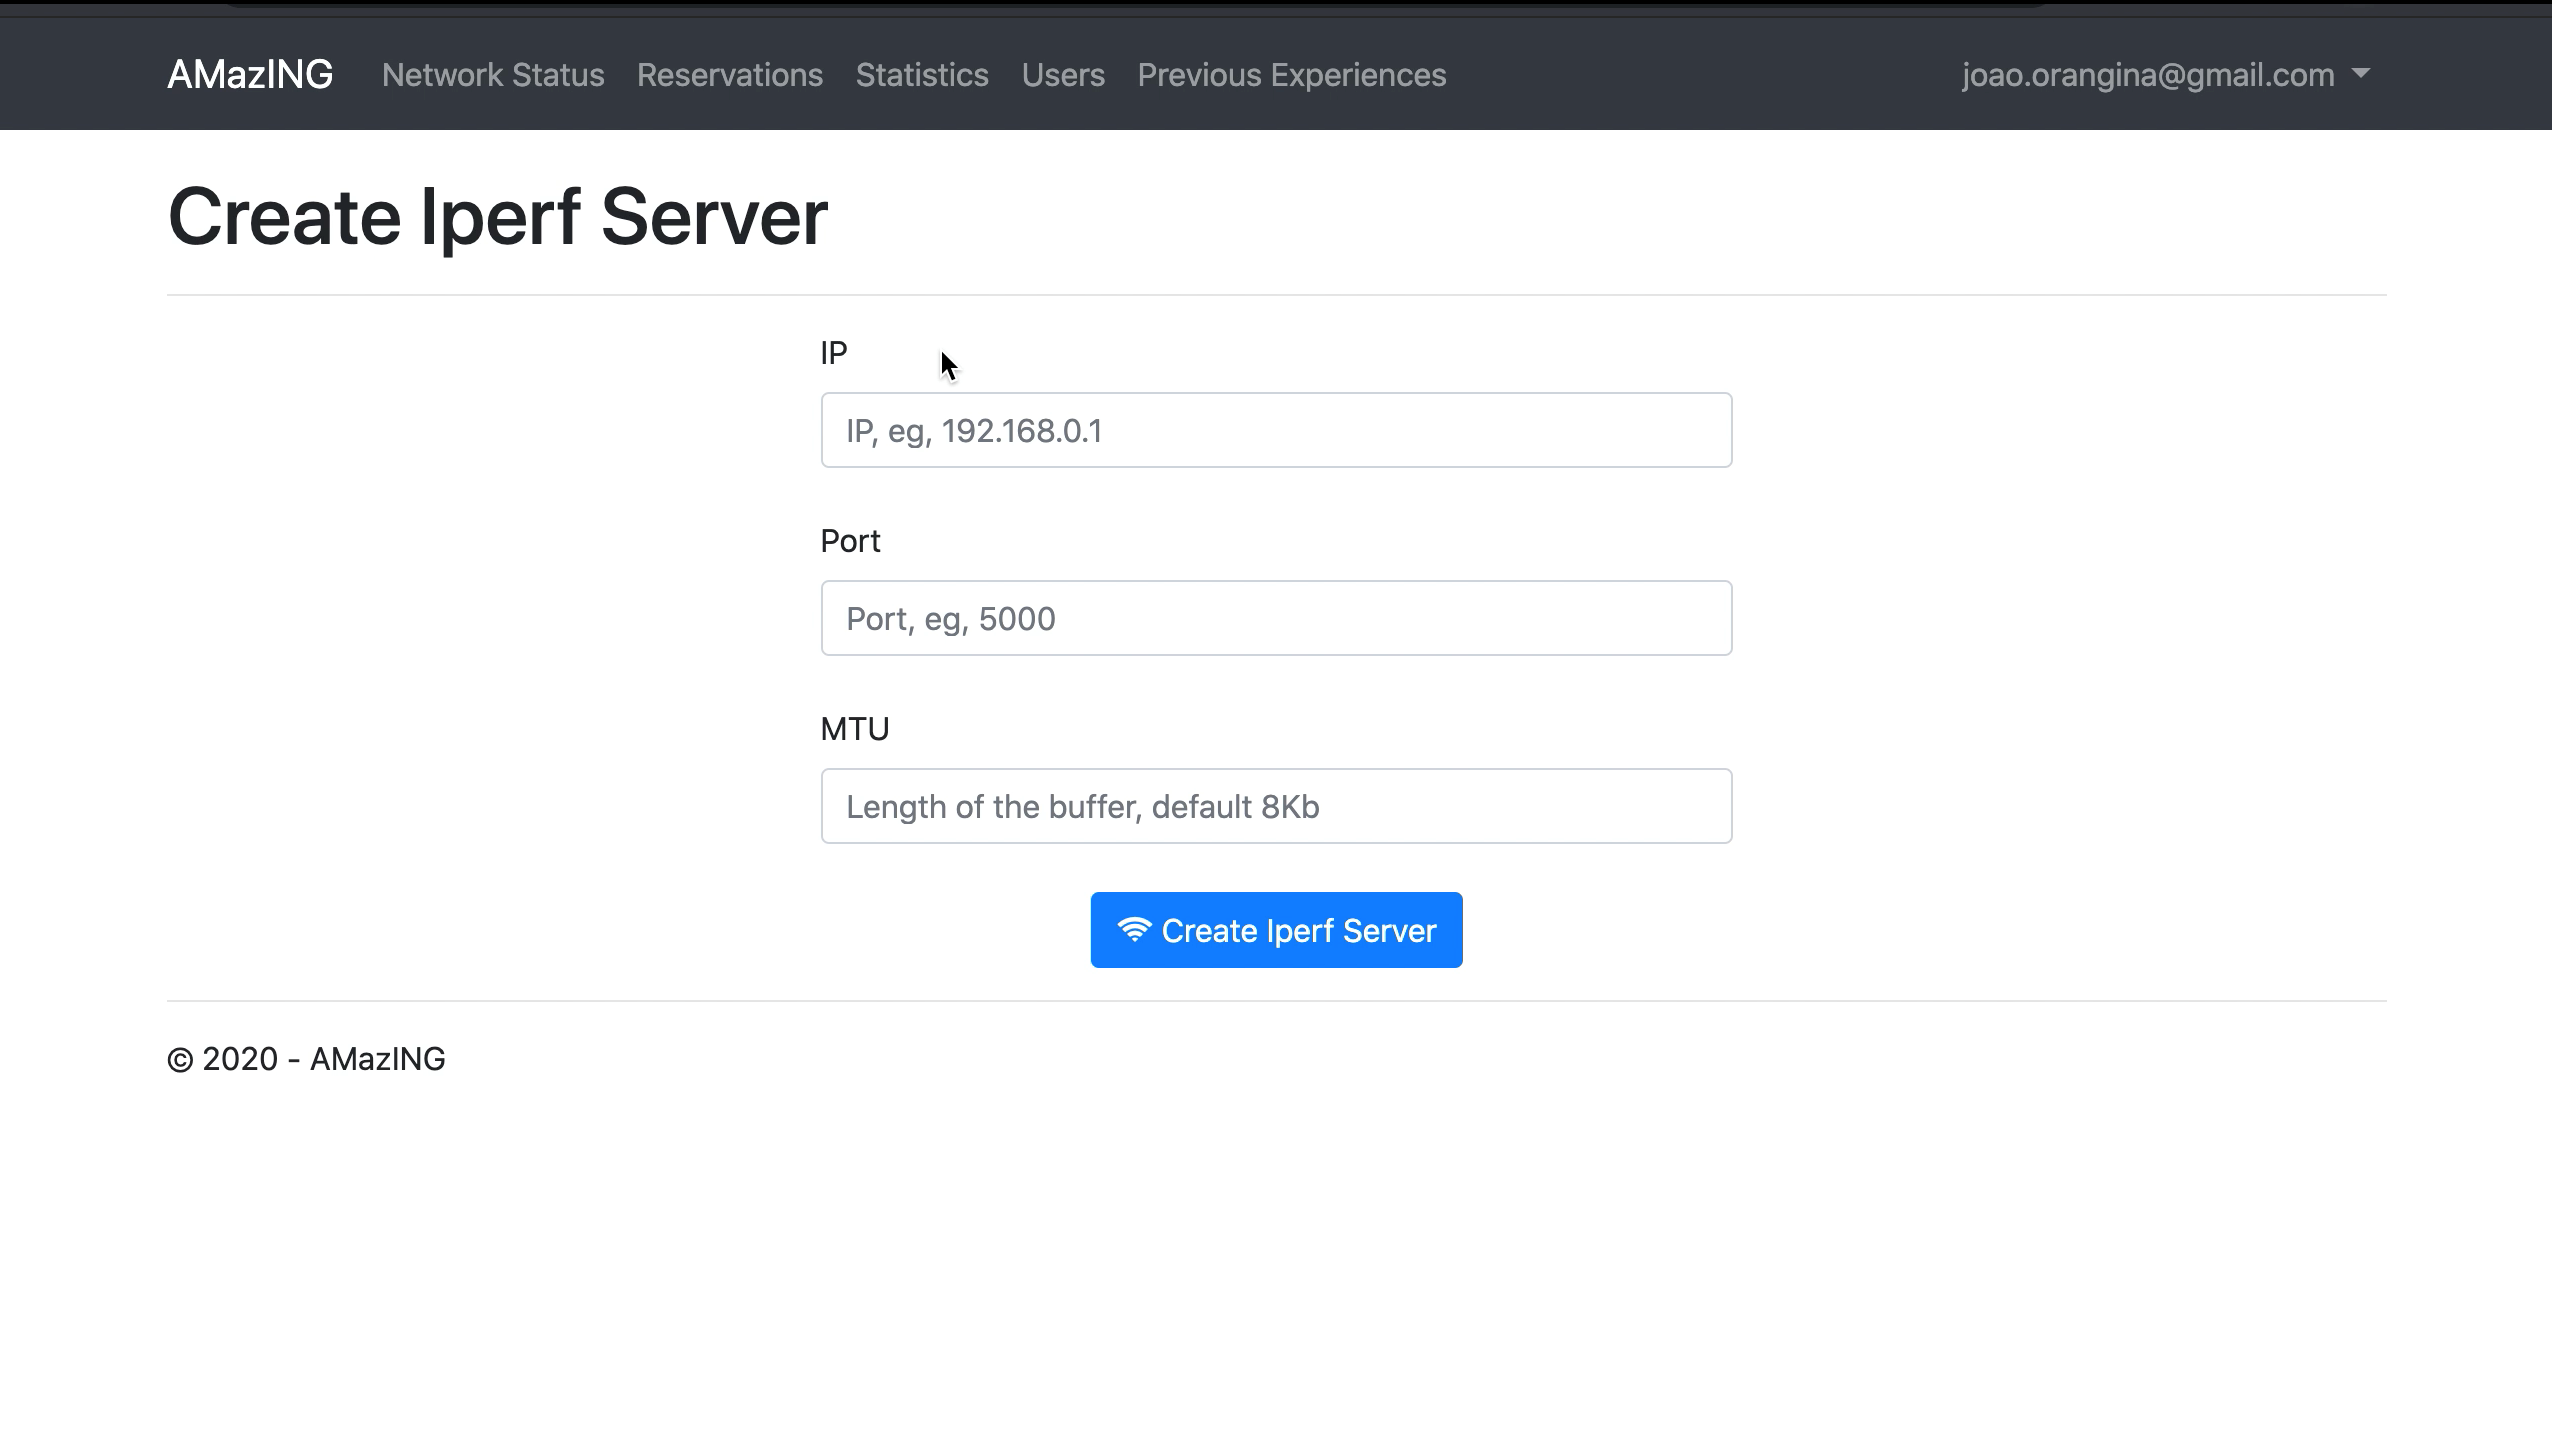
\includegraphics[width=0.7\textwidth]{images/create_iperfsv.png}
    \caption{Exemplo de criação de um Iperf Server}
    \label{fig:iperfserv}
\end{figure}

\subsection{Scan}
Utilizando este template, é possível realizar um scan através das interface de rede wireless, sem que seja necessário executar qualquer tipo de comando. O Frontend envia o pedido de scan para a API e esta encaminha-o para o APU, onde é traduzido para comandos shell. Terminado o scan, a informação é retornada e o frontend renderiza uma tabela na página das APUs com a informação obtida.\newline
Após ter feito scan, o utilizador pode carregar no botão para se conectar a uma das redes encontradas. Se a rede selecionada for aberta, pode conectar-se diretamente sem que seja necessário qualquer password. No caso de a rede ser protegida, o utilizador é redirecionado para uma página em que pode inserir a password da rede de modo a que se possa conectar a esta.
\begin{figure}[!ht]
    \centering
    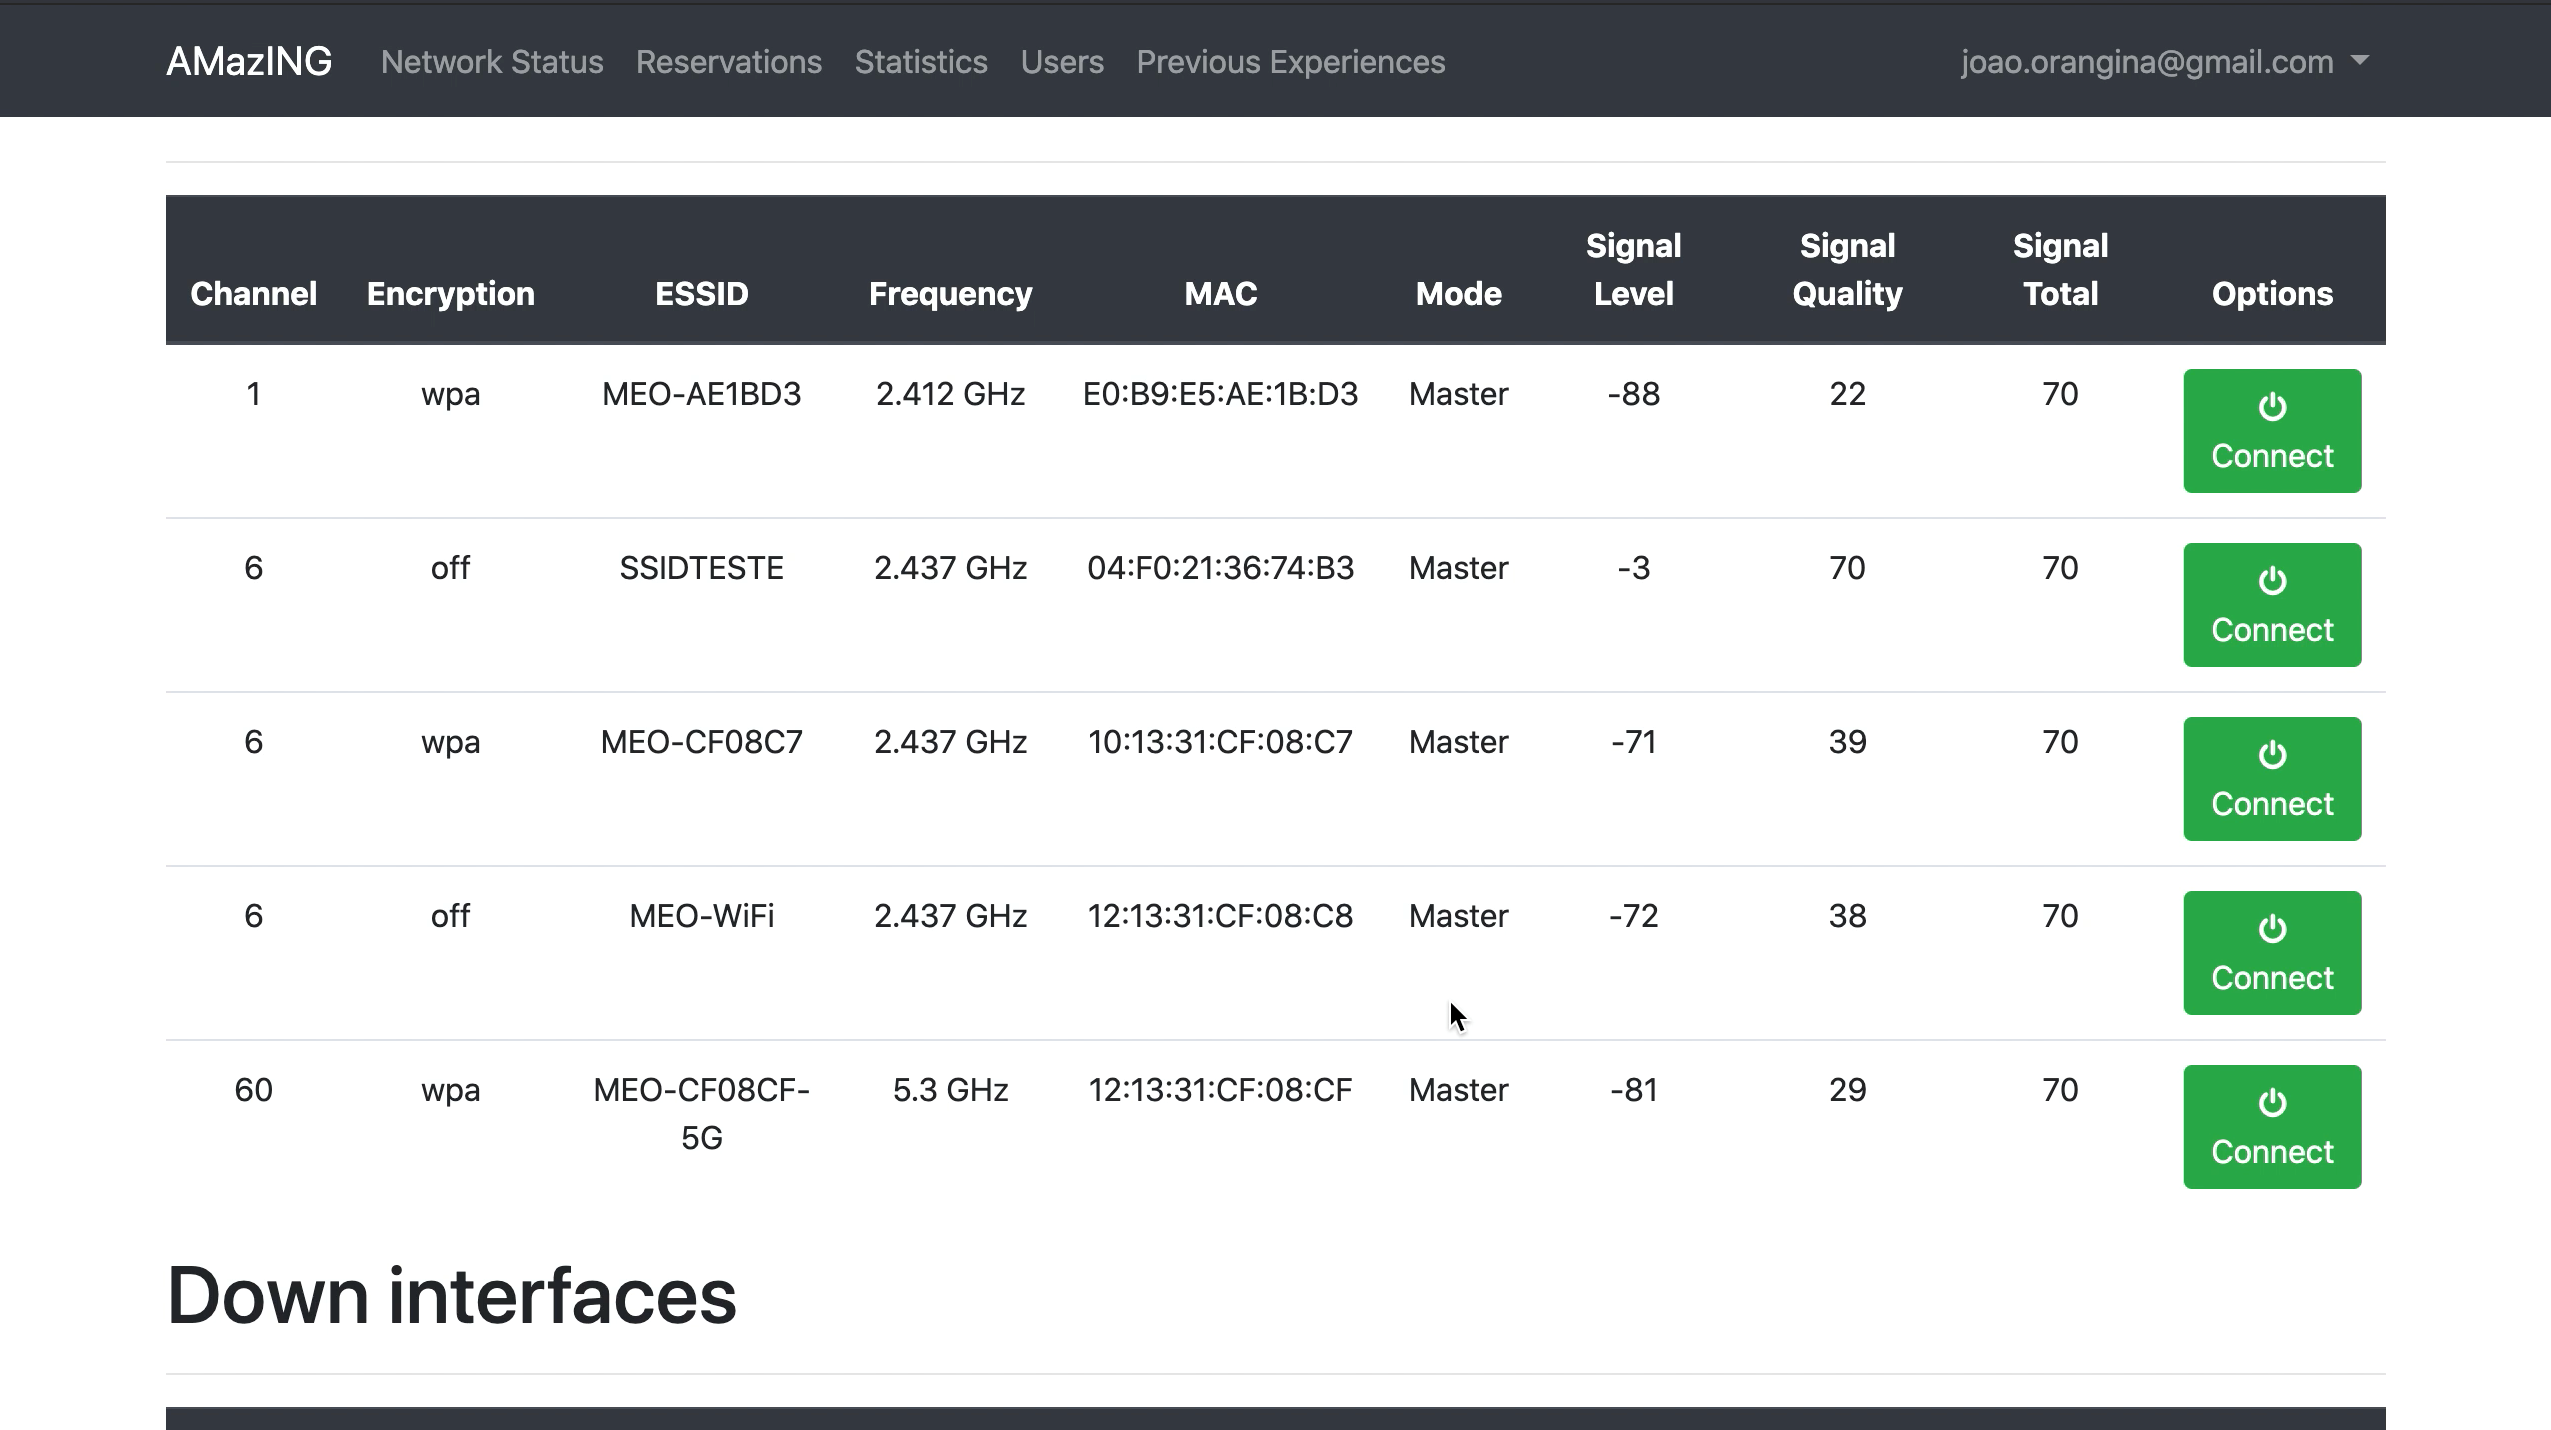
\includegraphics[width=0.9\textwidth]{images/scan_results.png}
    \caption{Exemplo de um scan}
    \label{fig:scannetwork}
\end{figure}

\subsection{WebSSH}
Uma das features que foi considerada das mais importantes para os utilizadores avançados era a utilização direta das APUs. Isto é, a possibilidade de aceder às mesmas de forma direta através da linha de comandos, sem necessidade de configurações extra. Para solucionar este problema, foi utilizada uma biblioteca de Python, o WebSSH. Esta biblioteca permite a criação de uma ligação aos APUs através de uma página web. Para que este serviço seja possível de utilizar, além do servidor de Django, que se encontra a correr de forma permanente, existe um segundo servidor, mais pequeno, que corre uma instância de Python, sendo lançado através de um Dockerfile.\hfill\break

\begin{figure}[!ht]
    \centering
    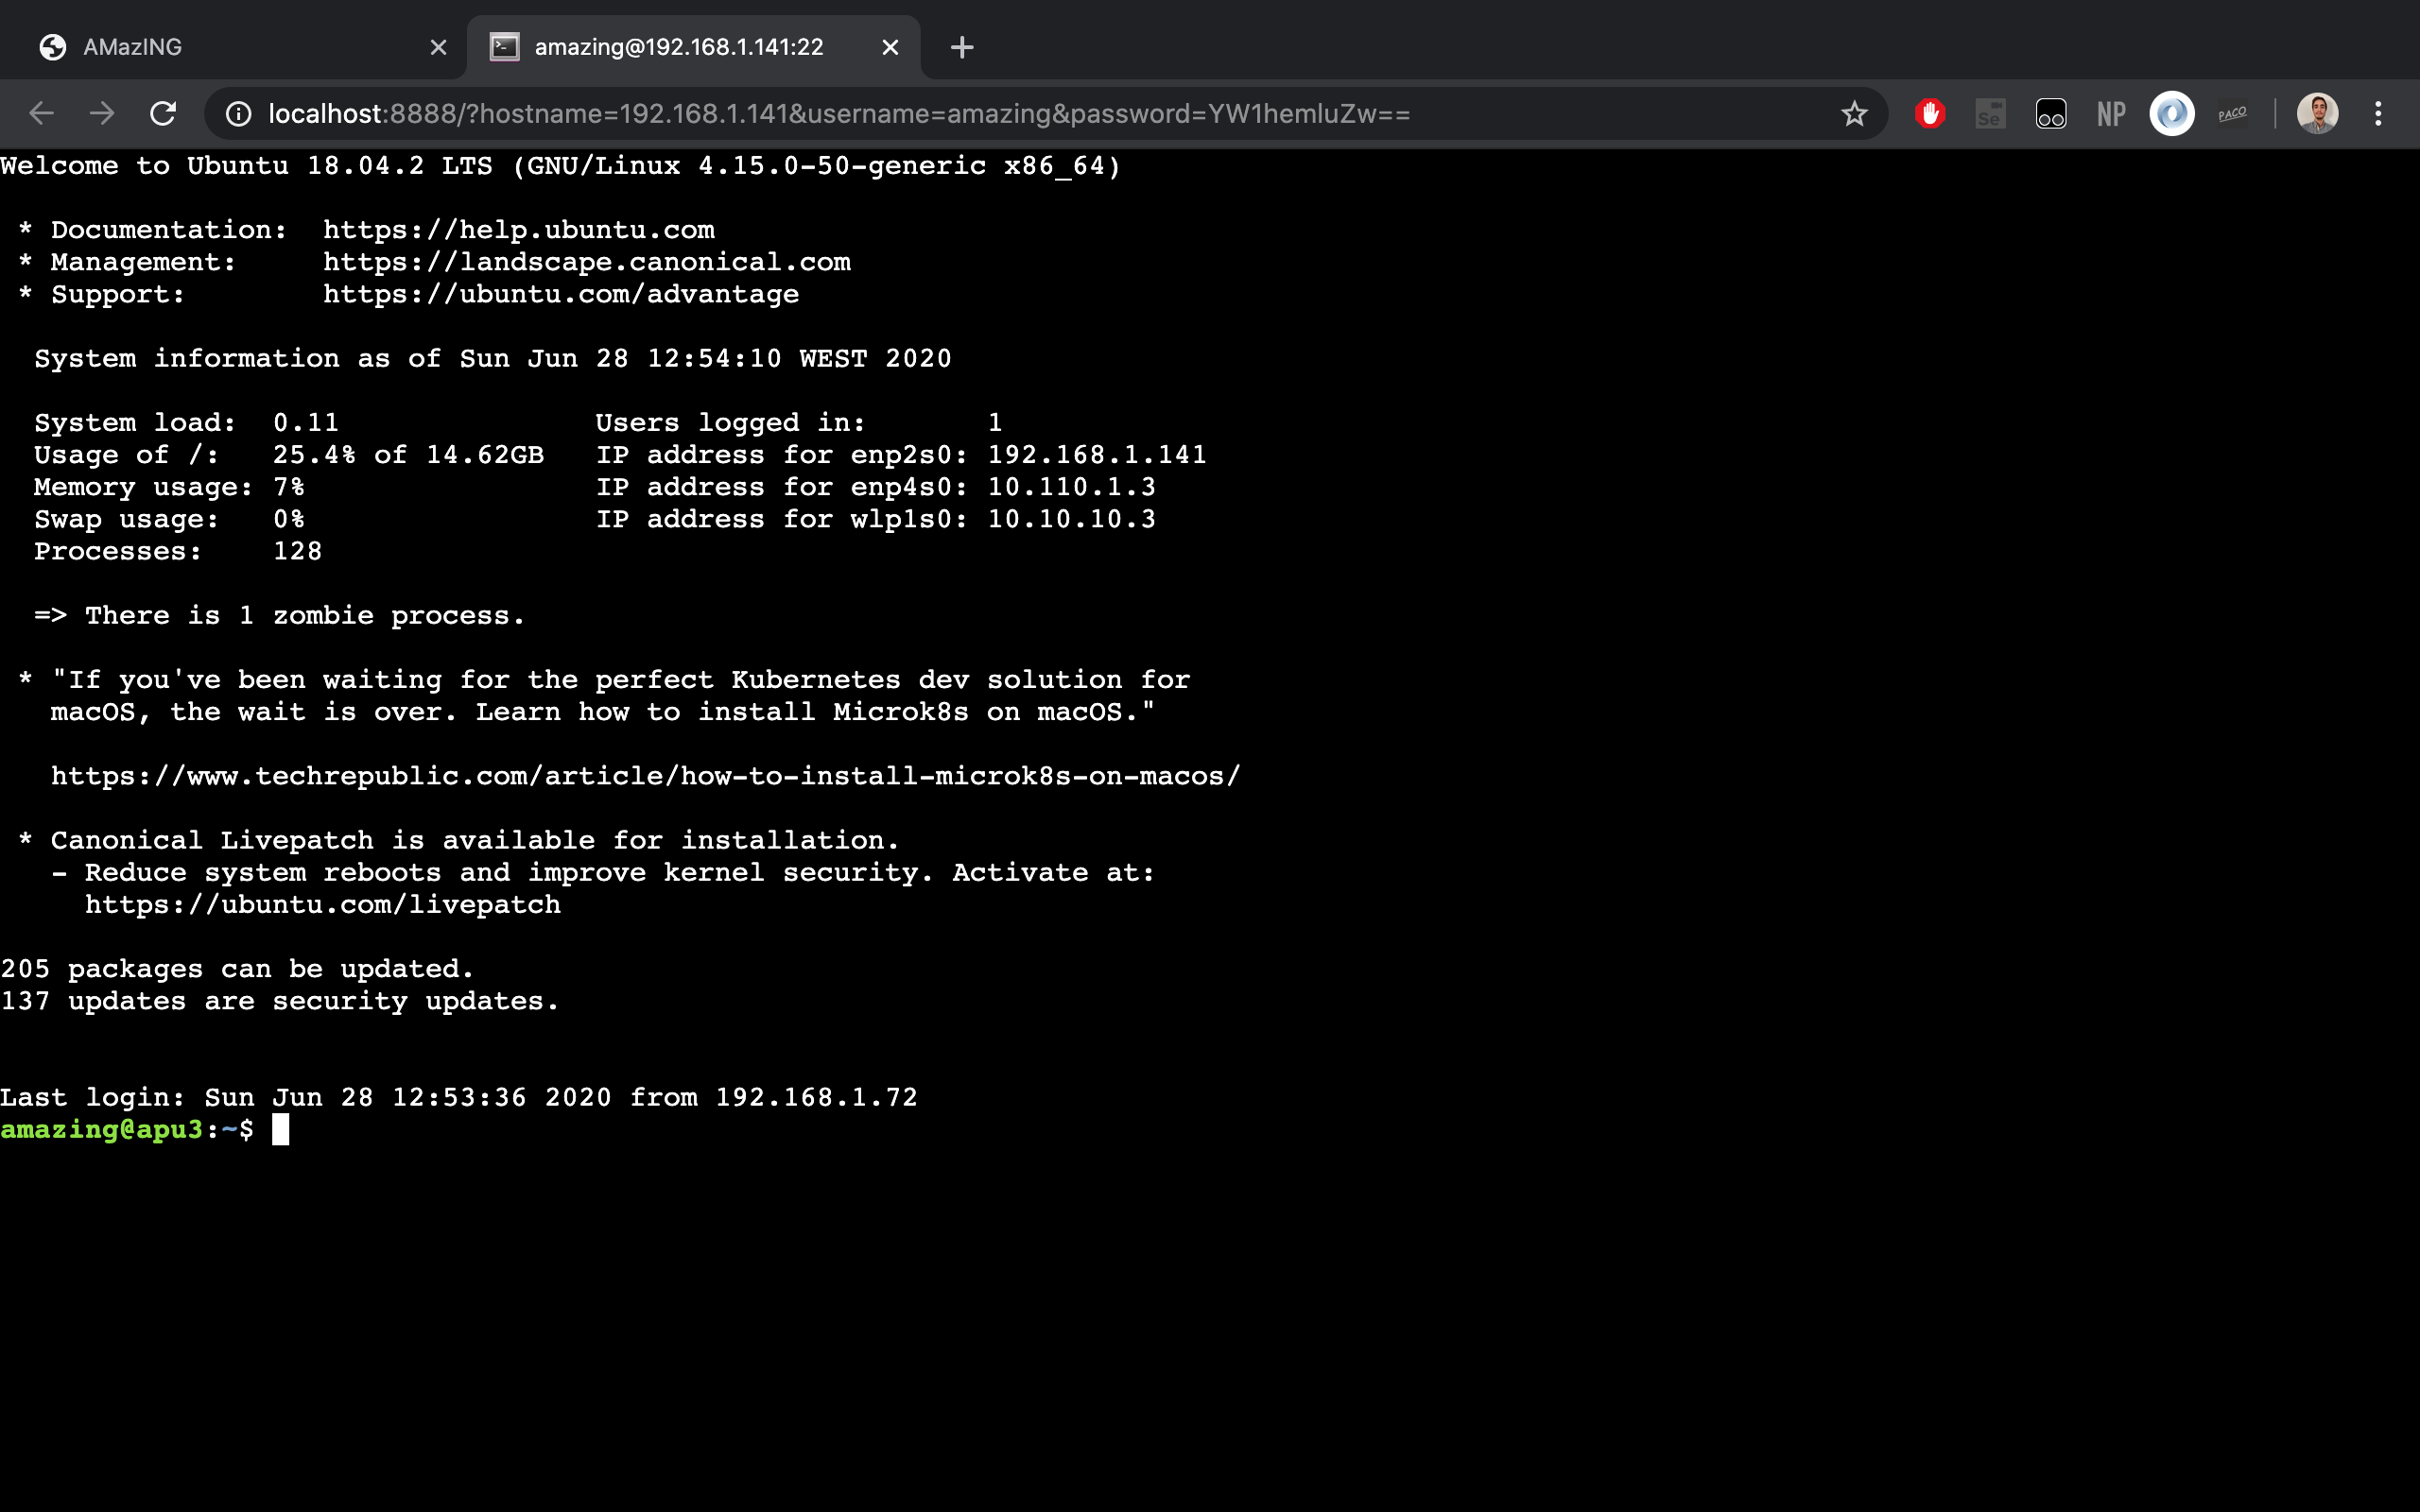
\includegraphics[width=0.9\textwidth]{images/webssh.png}
    \caption{Exemplo de um túnel ssh via broswer}
    \label{fig:ssh}
\end{figure}

\subsection{Agendamento de experiências}
Um dos requisitos para esta plataforma era a possibilidade de agendar uma experiência. De modo a tornar isto possível, foi desenvolvido um calendário para ser associado à plataforma. Este calendário possui informação sobre todas as experiências que já ocorreram e vão ocorrer.
\subsubsection{Visualização de experiências}
O utilizador pode consultar as experiências agendadas por dia dirigindo-se ao separador do calendário existente na navbar.\newline
No calendário disponível, o utilizador pode consultar todas as experiências realizadas na plataforma, podendo fazer variar o mês, o dia e o ano de forma simples e intuitiva, através do painel lateral disponível.
\newpage
\begin{figure}[!ht]
    \centering
    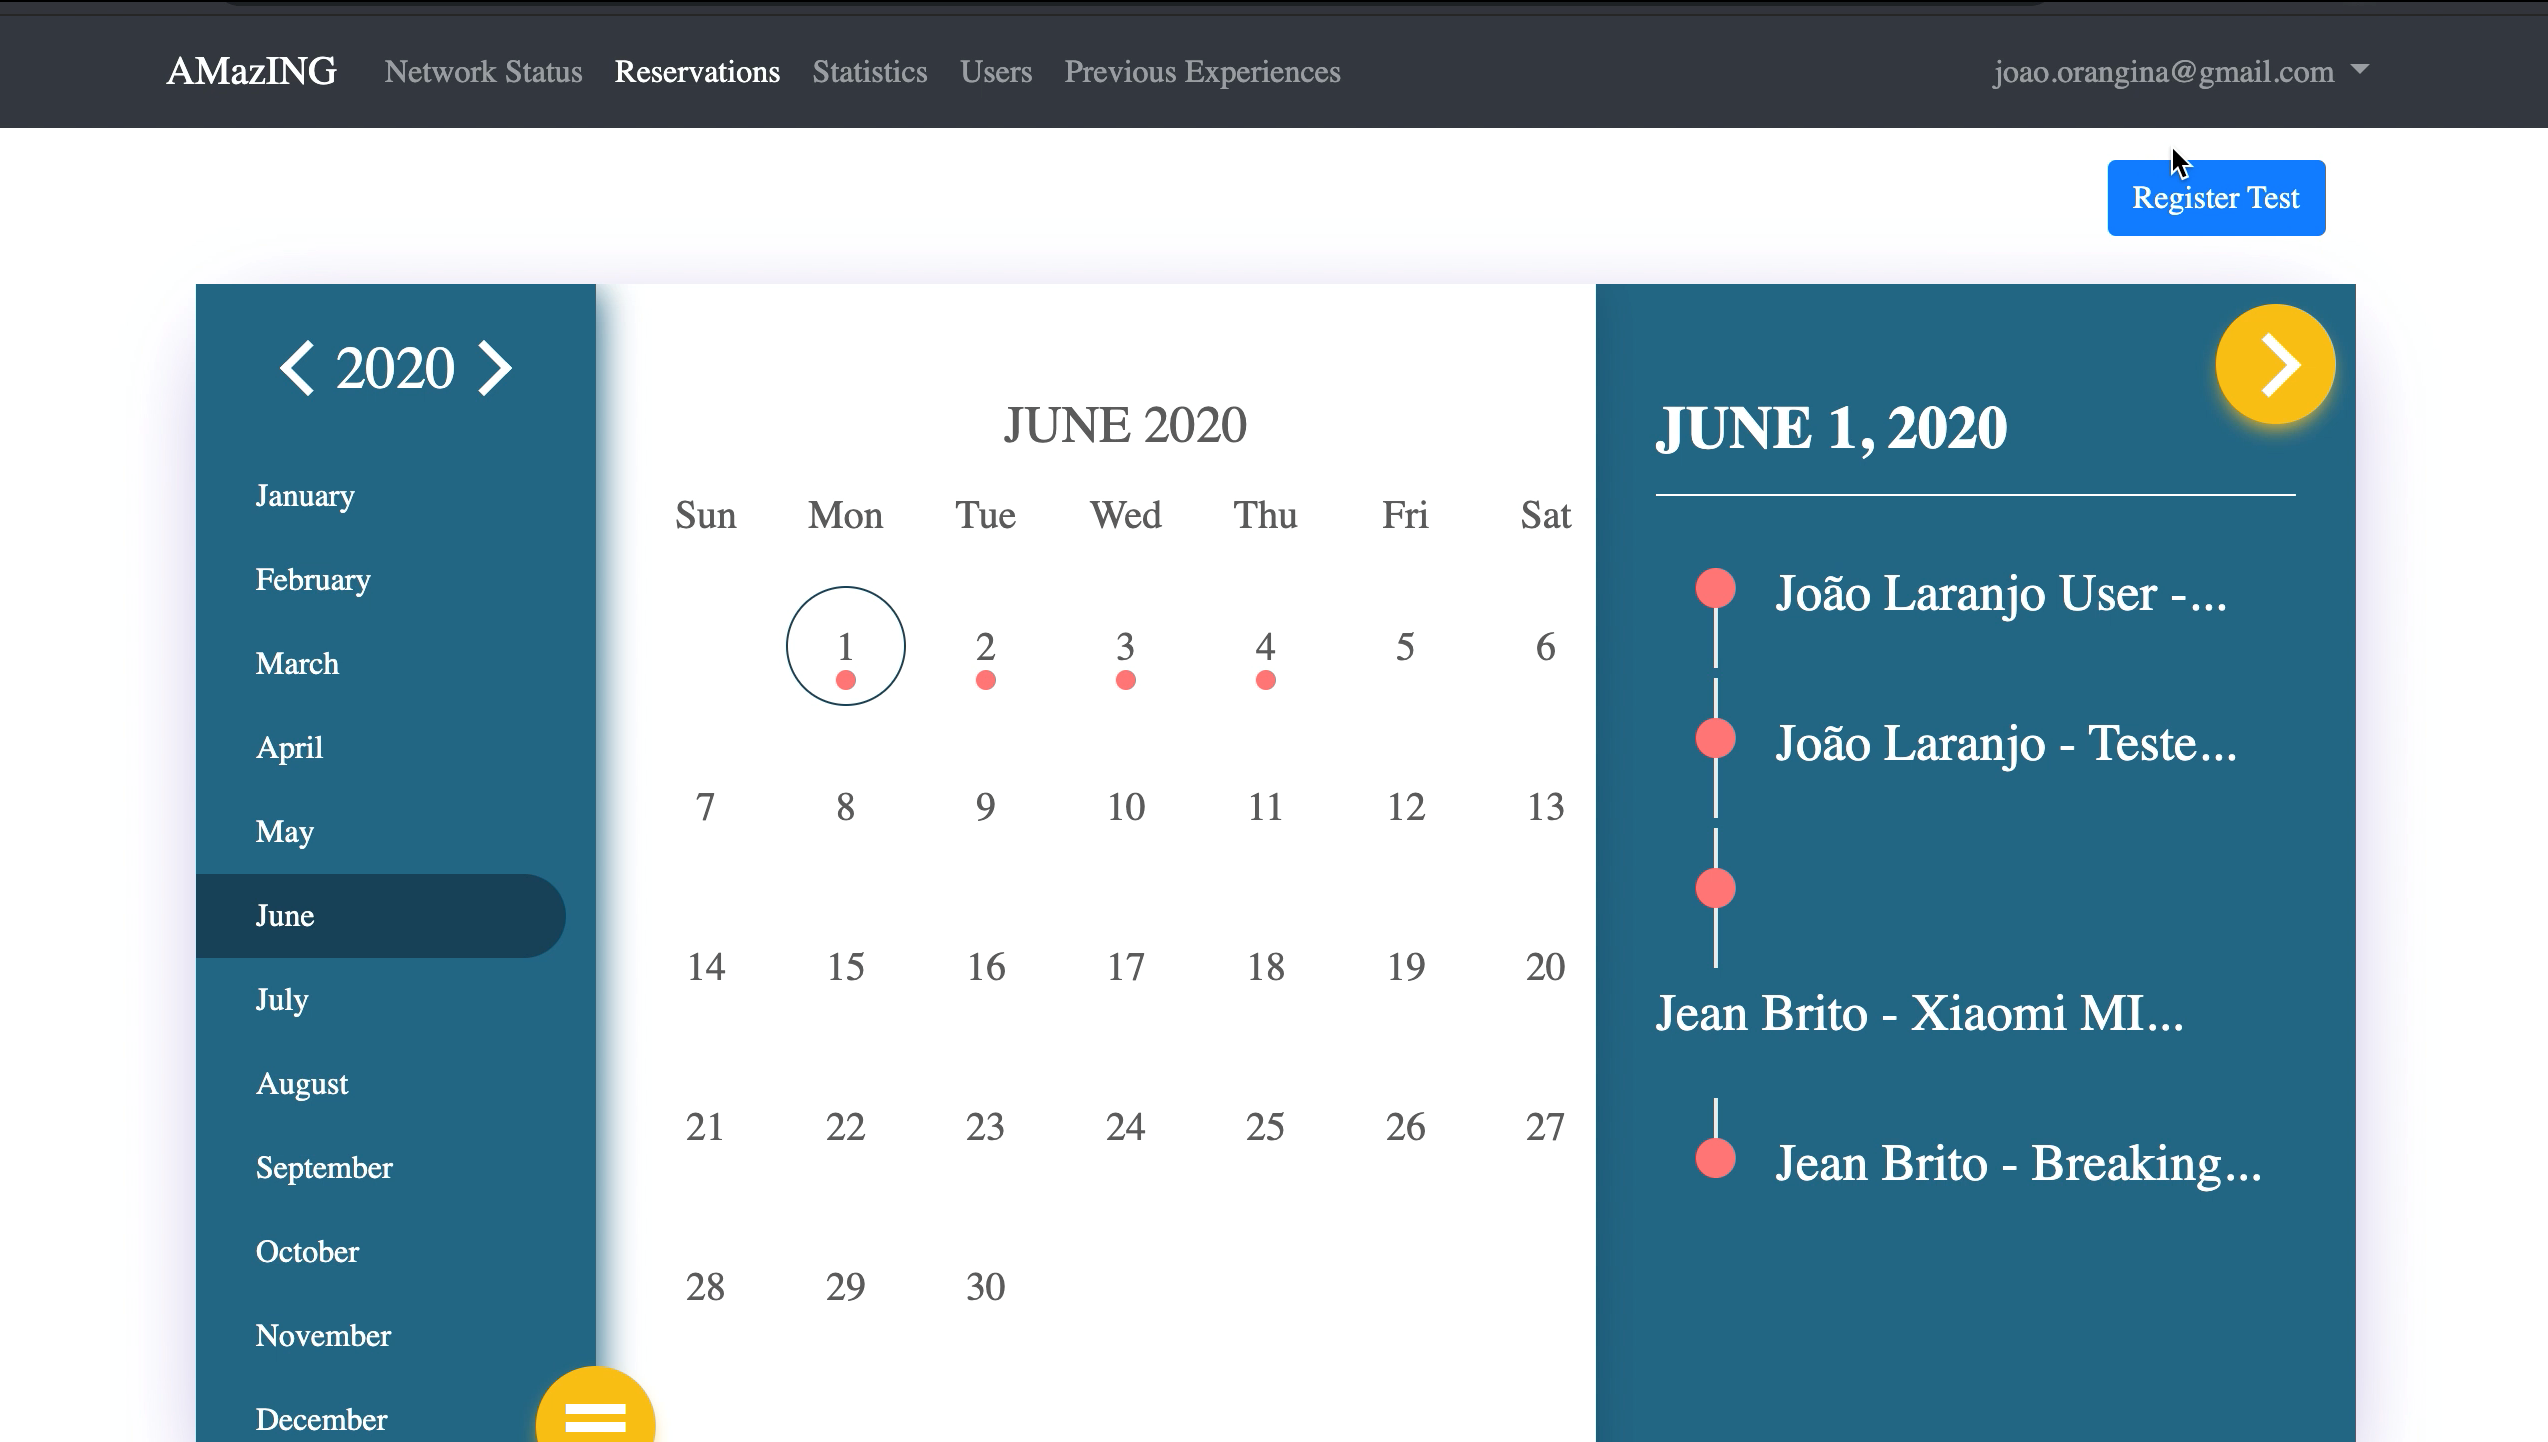
\includegraphics[width=0.8\textwidth]{images/calendar.png}
    \caption{Calendário}
    \label{fig:calendar}
\end{figure}

\subsubsection{Marcação de experiências}
Ainda neste separador, o utilizador possui um botão que o direciona para um formulário que permite que este registe um horário em que quer agendar a experiência. A informação é validada previamente no Django, sendo depois  enviada para a API, onde é validada toda a integridade e disponibilidade de realização de experiências.
\begin{figure}[!ht]
    \centering
    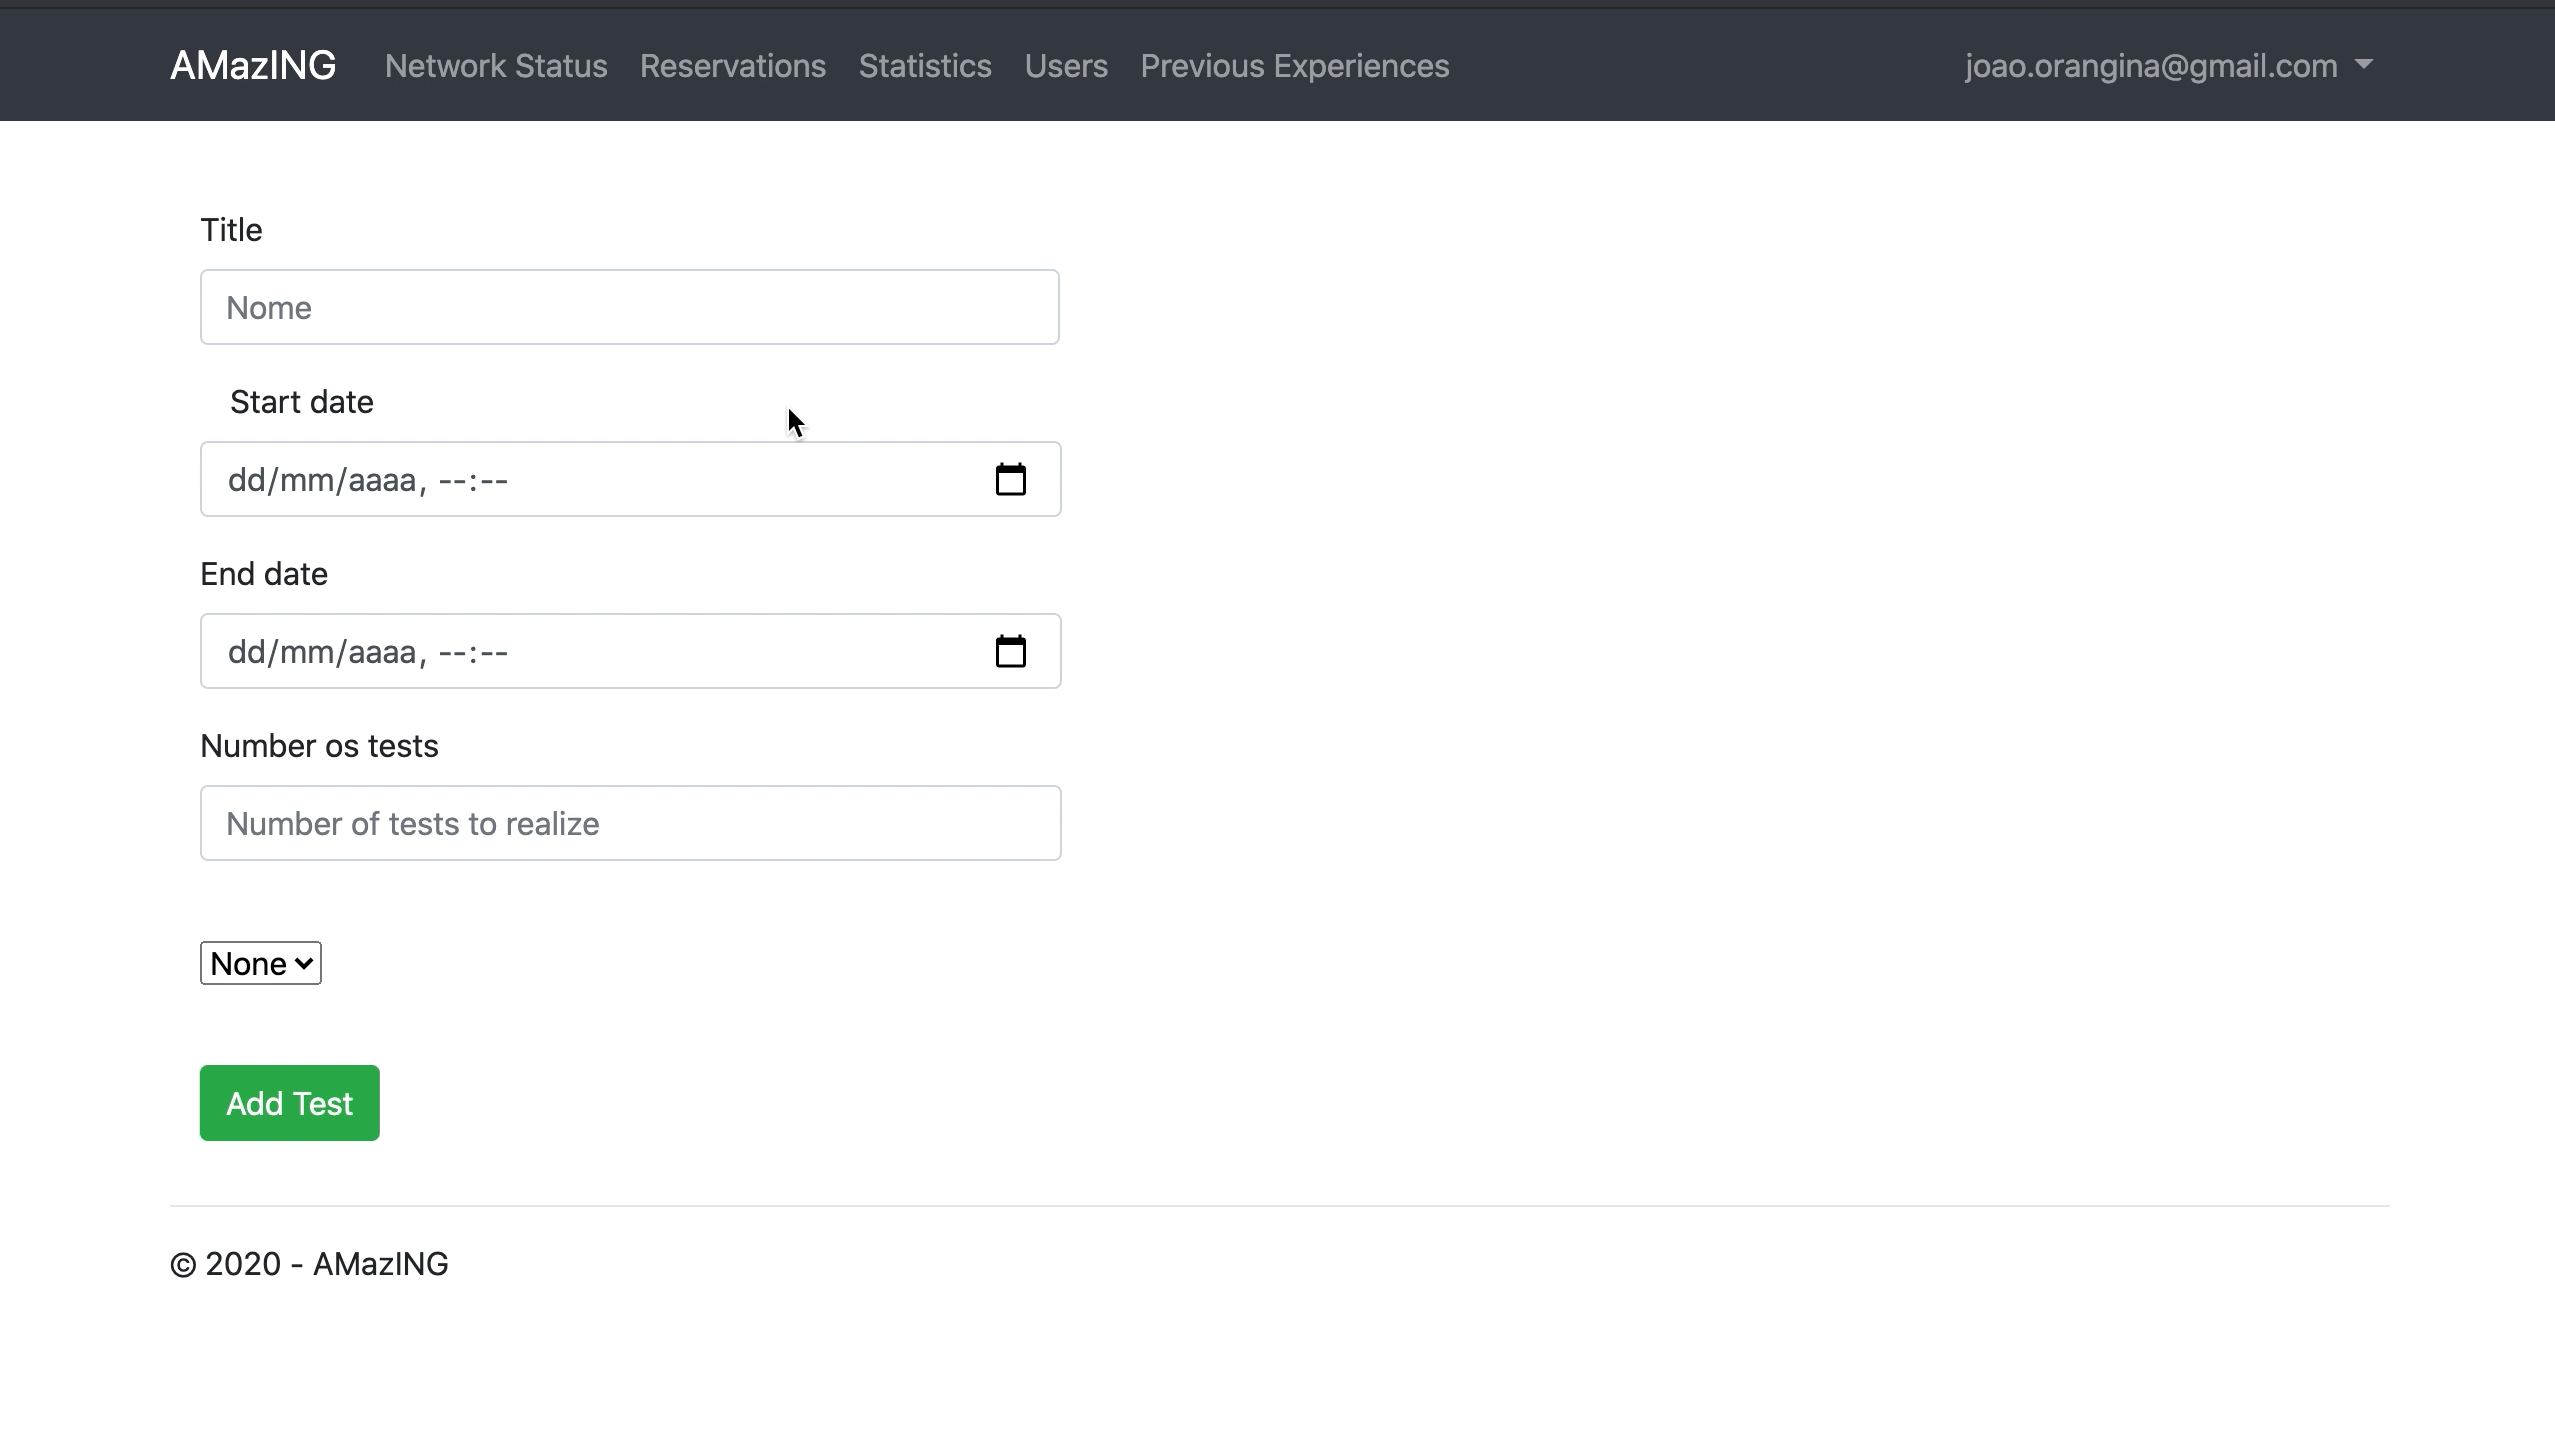
\includegraphics[width=0.8\textwidth]{images/make_reservation.png}
    \caption{Realização de uma reserva}
    \label{fig:reserva}
\end{figure}

\subsection{Experiências realizadas}
Além das vistas web mencionadas anteriormente, cujo objetivo é a gestão e agendamento de experiências que estão a acontecer ou vão acontecer, existe também um painel específico que contém informação sobre experiências passadas.\newline
Este painel mostra as experiências de um determinado utilizador ao longo do tempo. Quando o utilizador clica no botão de informações, este mostra as informações relativas às experiências, desde a sua data de ocorrência ao estado final.
É de notar que a imagem acima demonstra o painel visto como um administrador, no caso de o utilizador não ser administrador, a vista é similar, contudo, apenas apresenta as experiências do próprio utilizador.
\begin{figure}[!ht]
    \centering
    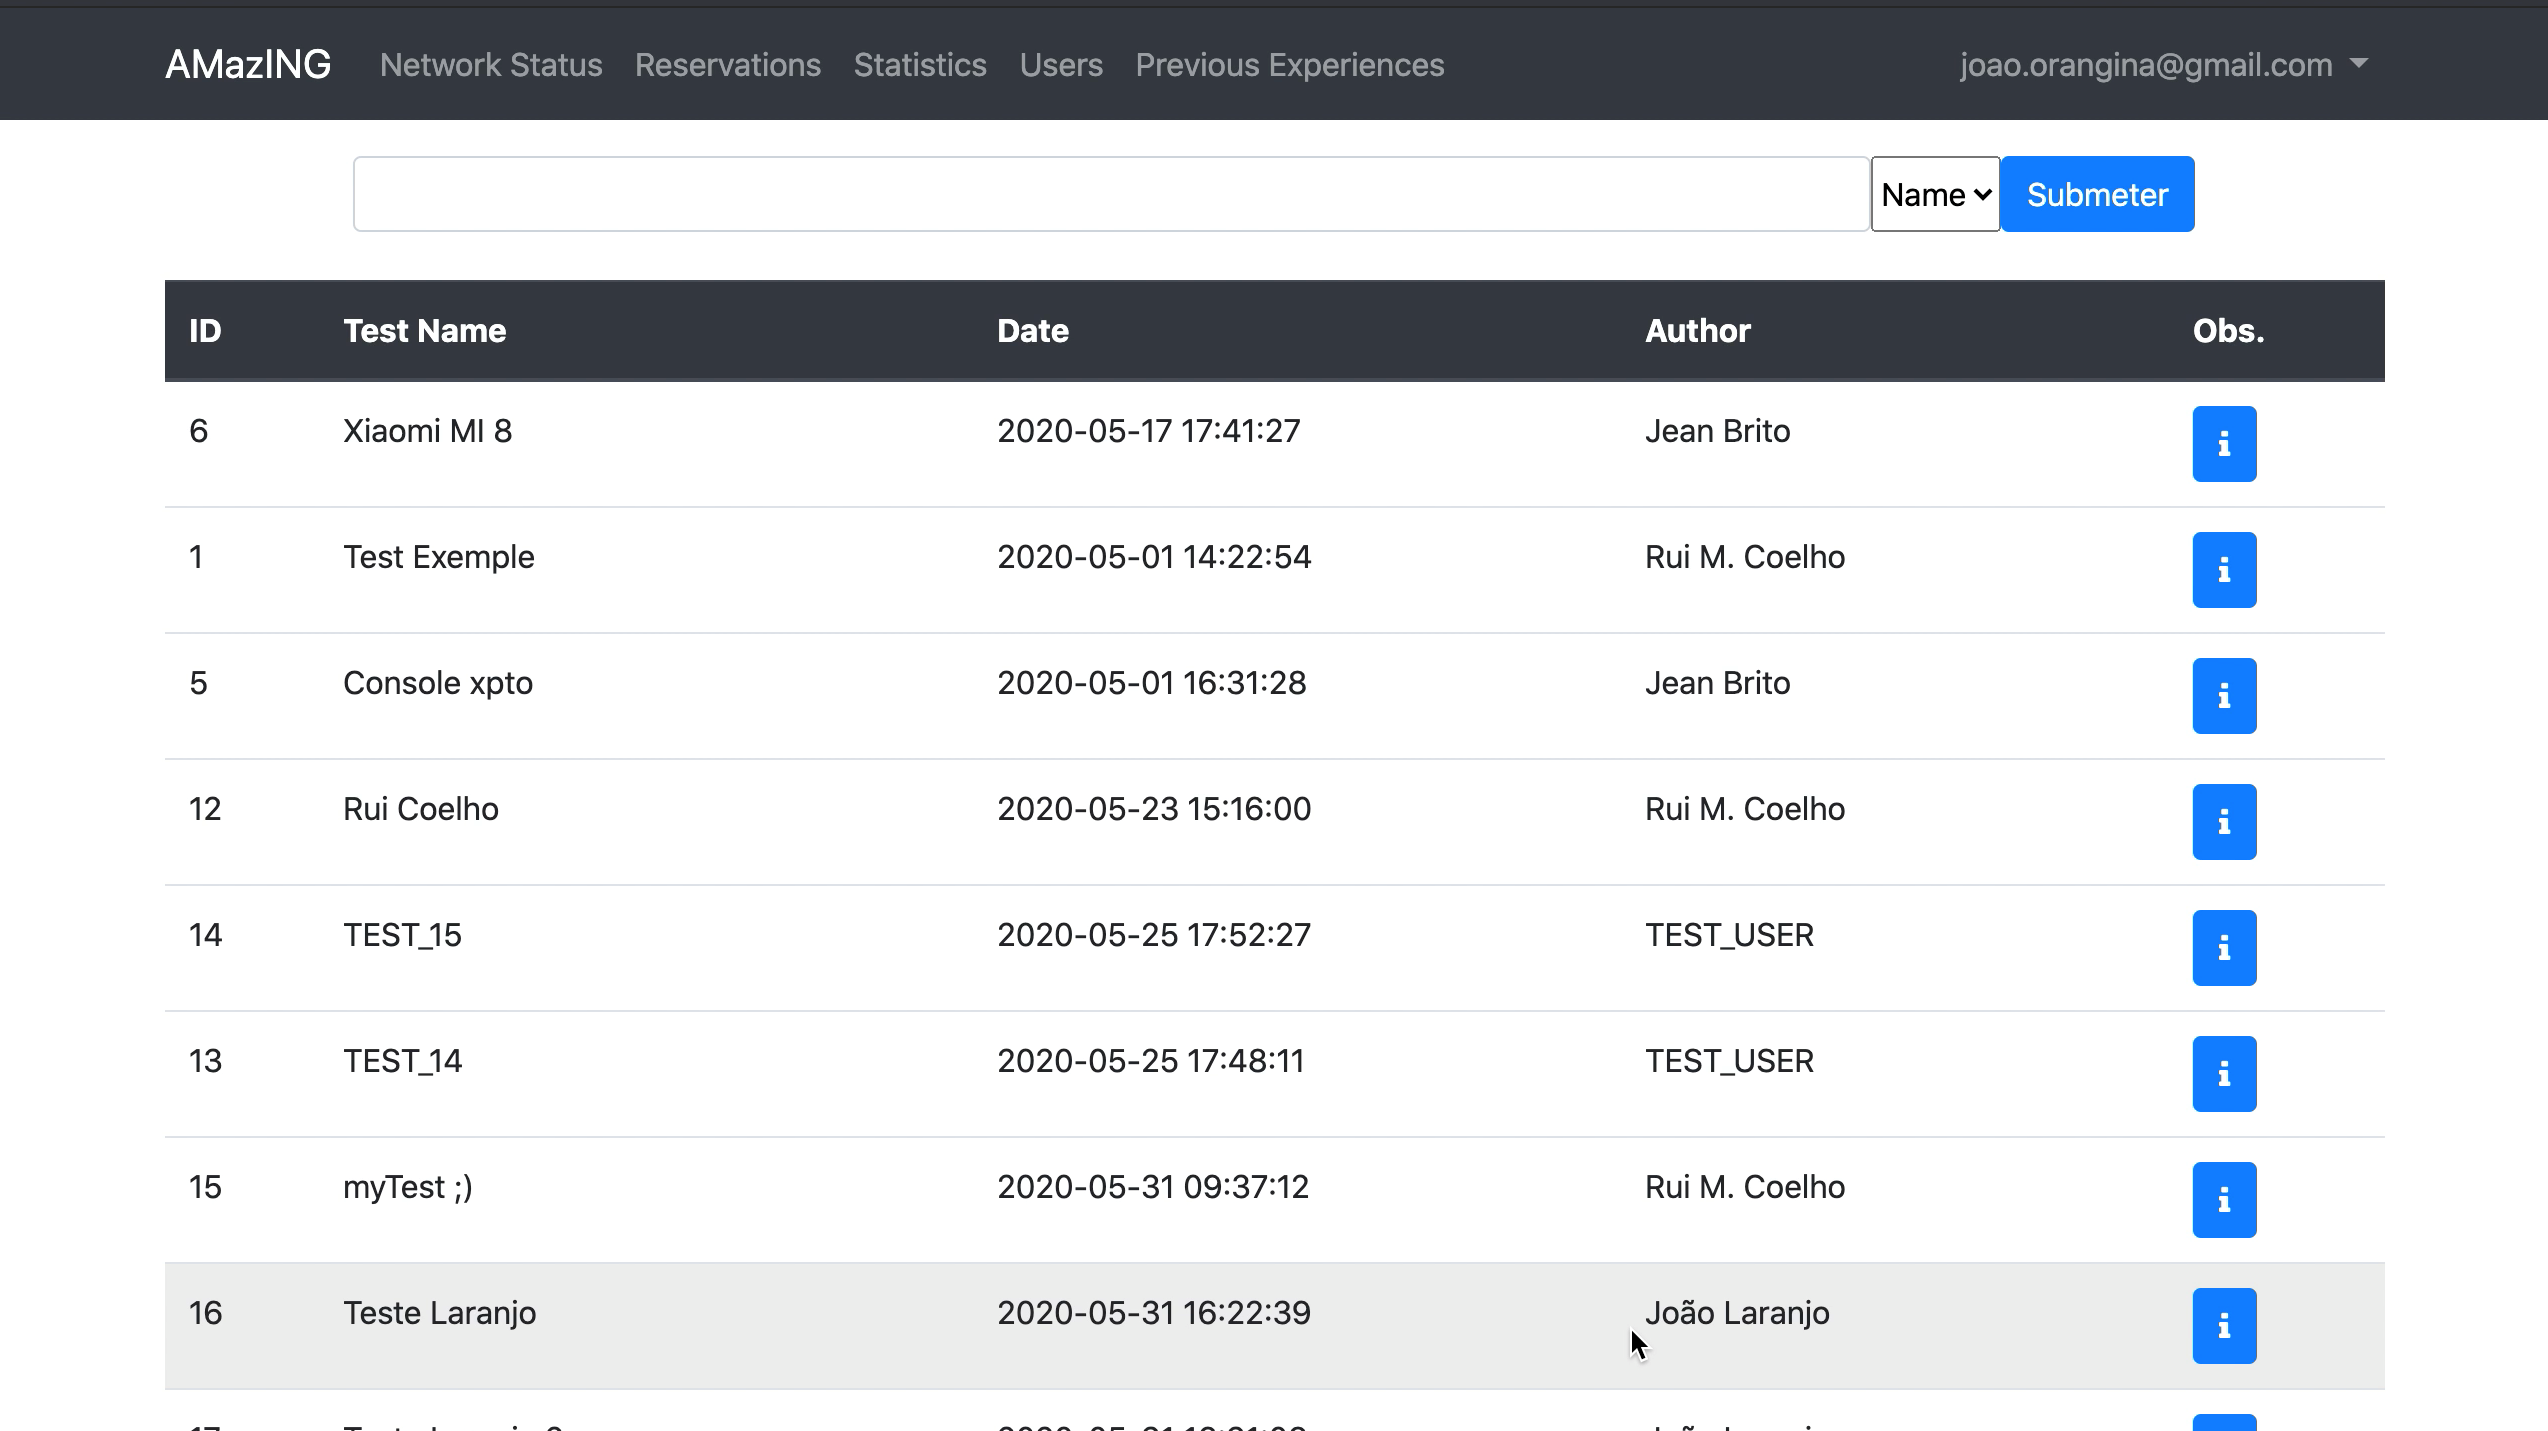
\includegraphics[width=0.7\textwidth]{images/previous_experiences.png}
    \caption{Histórico de experiências}
    \label{fig:historico}
\end{figure}

\subsection{Gestão de perfis}
Além de todas  as funcionalidades já mencionadas, surgiu a necessidade de gerir perfis. Como tal, cada utilizador tem um perfil associado que pode consultar e modificar tendo efetuado login. Como existem dois tipos de utilizadores, os avançados e os iniciantes, surgiu também a necessidade de solicitação de subida de nível.
\subsubsection{Visualização do perfil}
Como mencionado anteriormente, o utilizador pode, a qualquer momento (desde que tenha o login efetuado), visualizar o seu perfil. Dentro desse painel existem duas opções disponíveis, editar informações e solicitar subida de cargo (caso seja iniciante).
\begin{figure}[!ht]
    \centering
    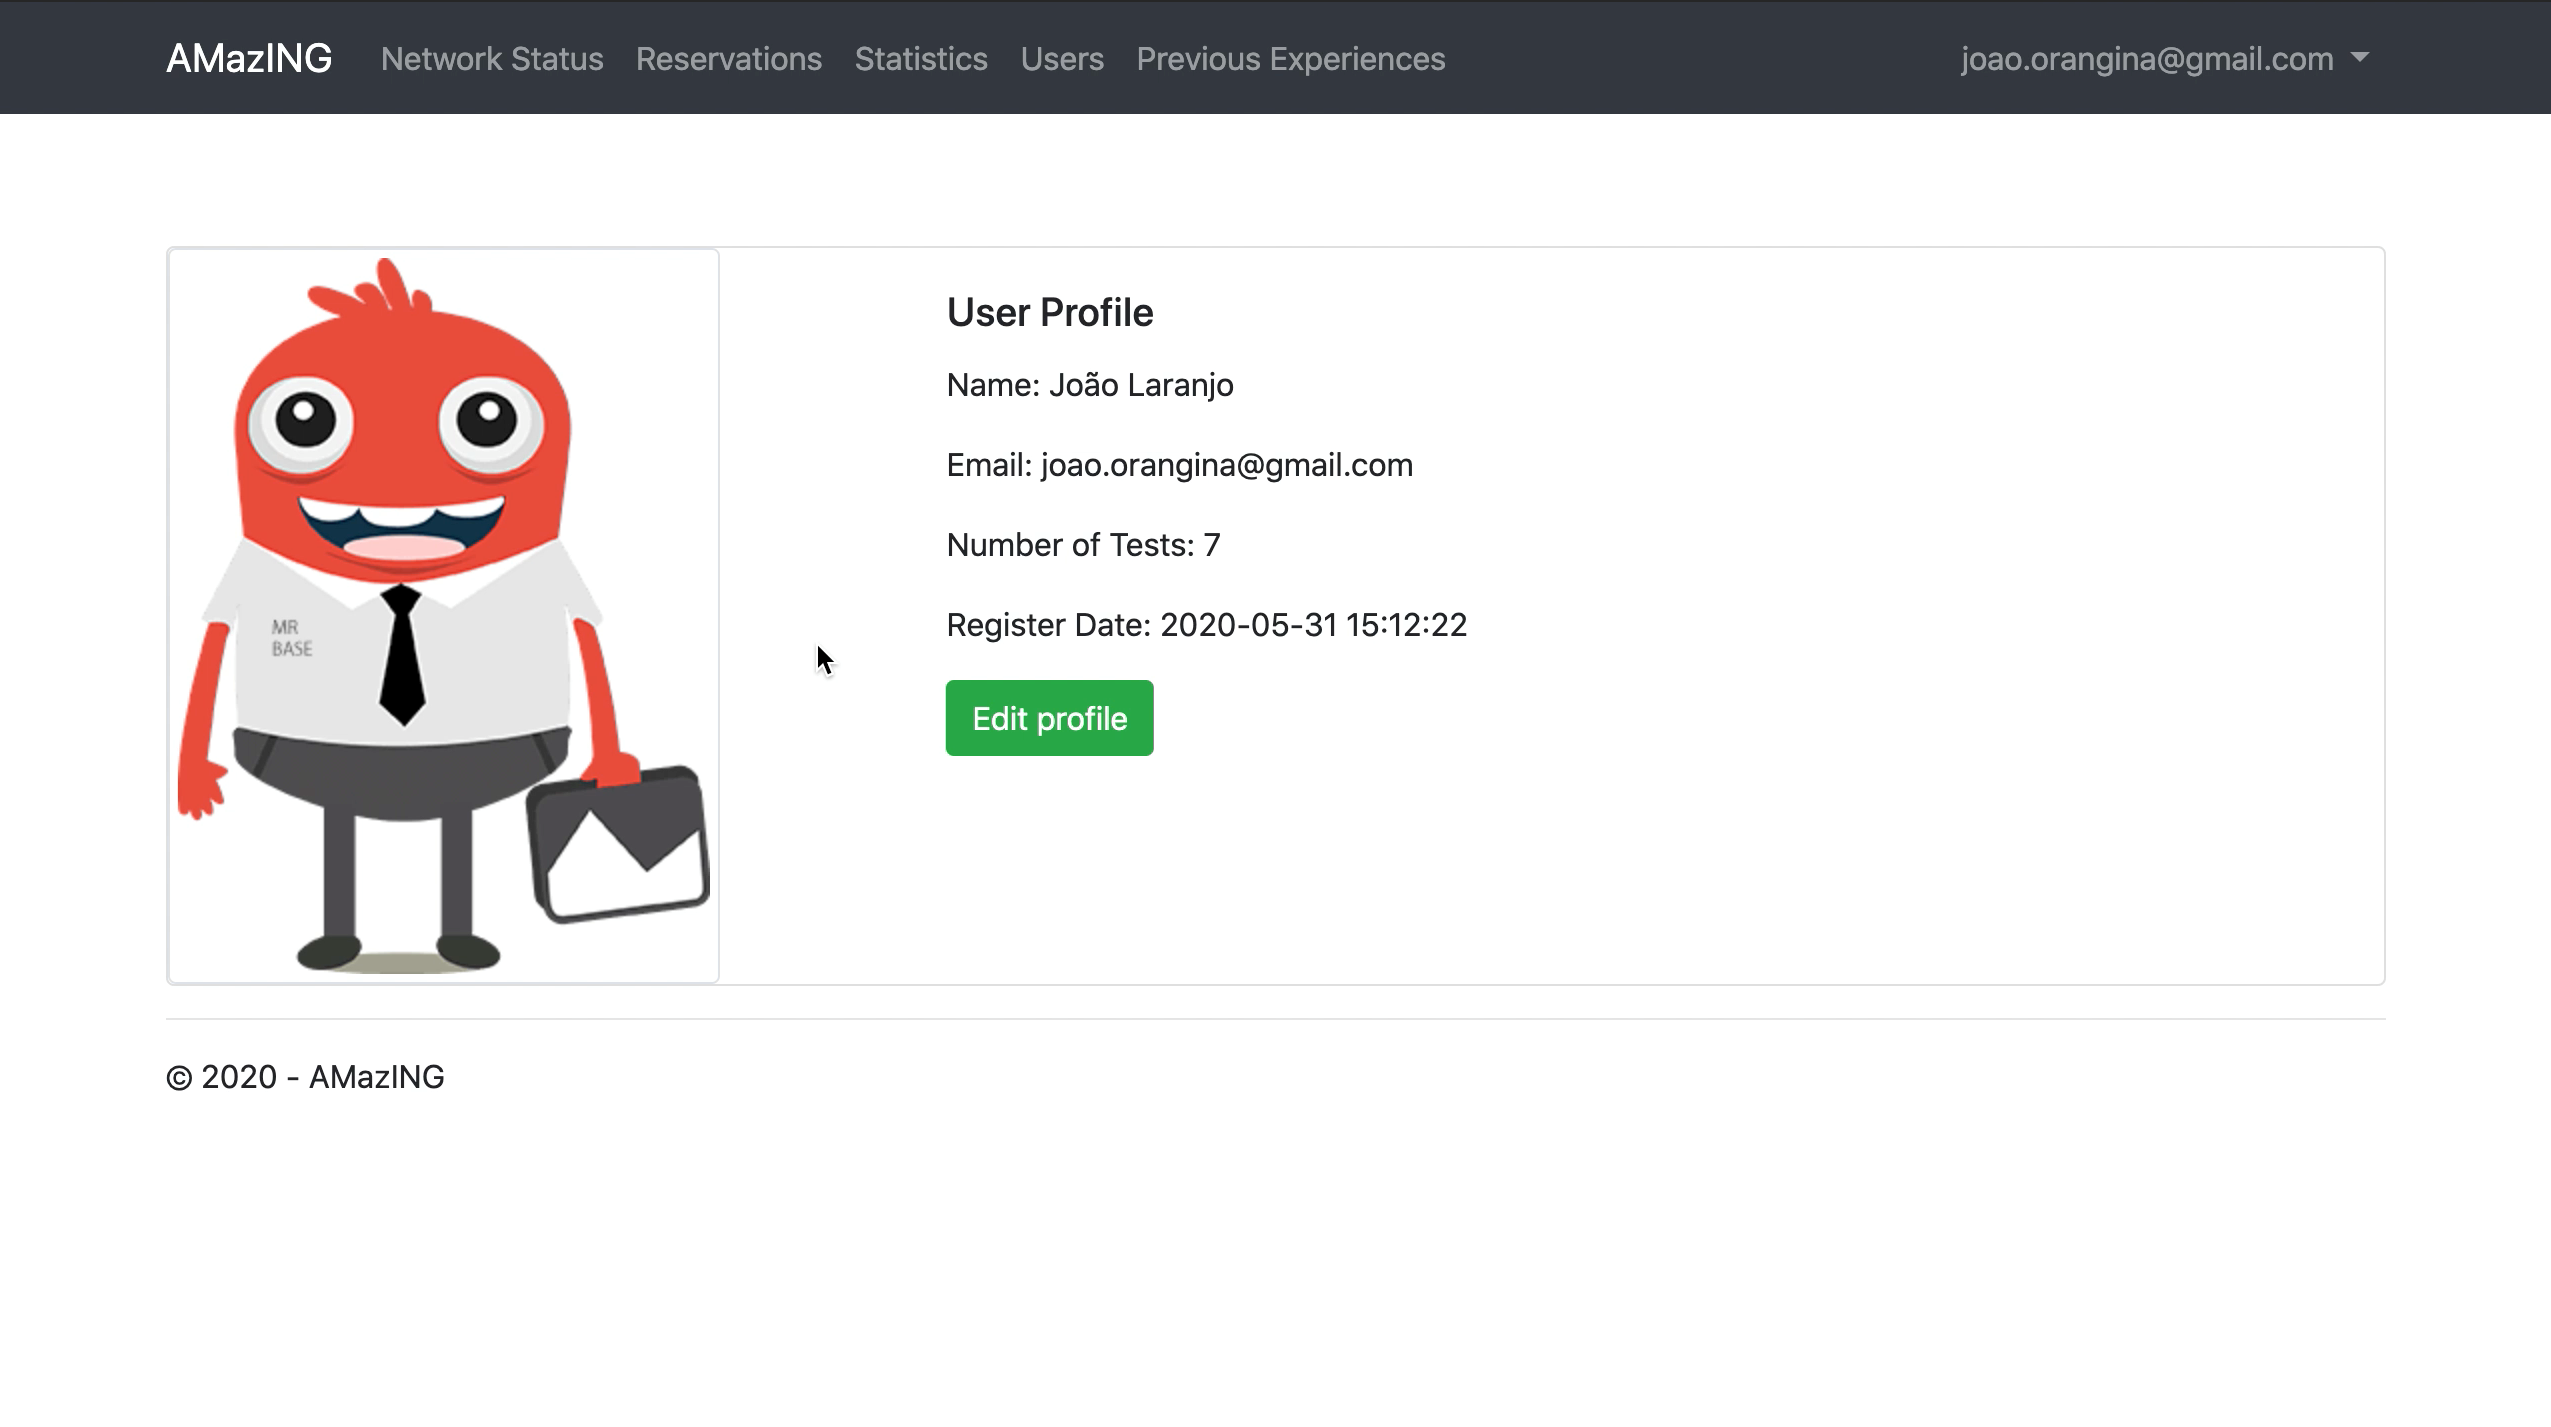
\includegraphics[width=0.9\textwidth]{images/my_profile.png}
    \caption{Vista de perfil}
    \label{fig:seeprofile}
\end{figure}
\subsubsection{Alteração de perfil}
Caso o utilizador deseje alterar o seu perfil, apenas tem que se dirigir ao painel de perfil e carregar no botão para alterar o mesmo. É importante mencionar que, devido ao modelo de dados escolhido, o utilizador pode apenas alterar o seu nome e fotografia, os outros dados não são passíveis de modificação.
\begin{figure}[!ht]
    \centering
    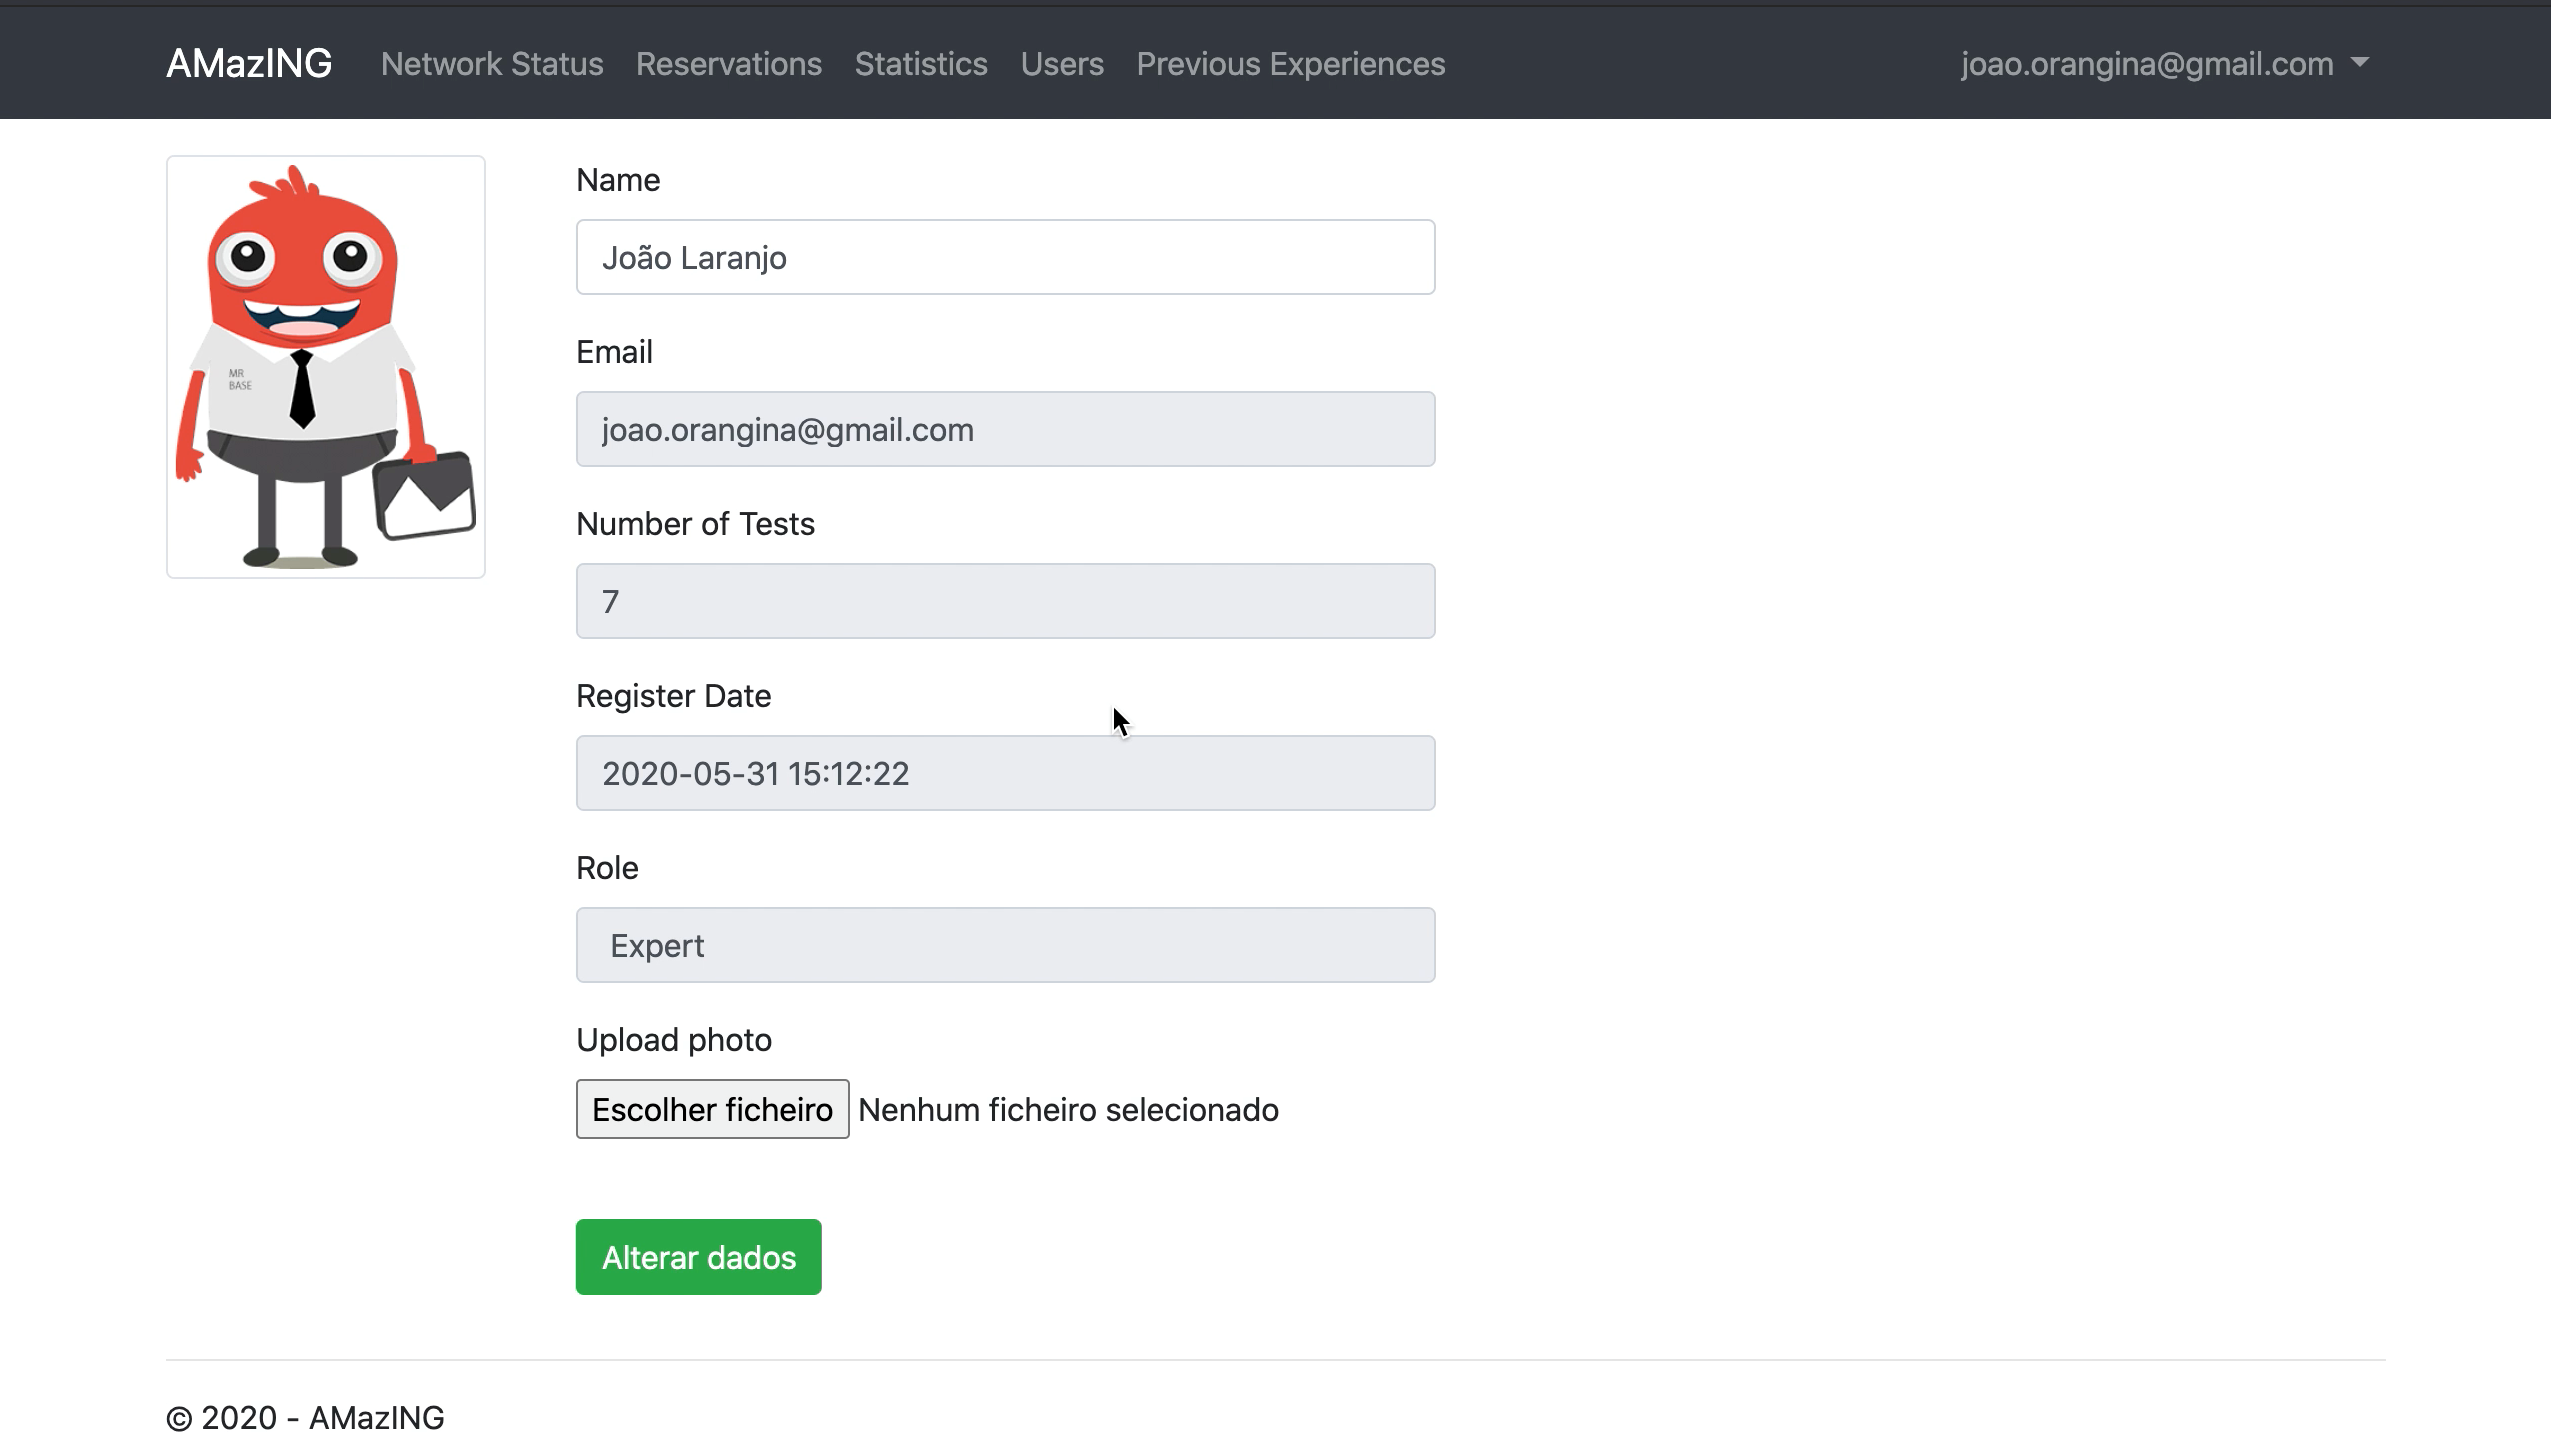
\includegraphics[width=0.9\textwidth]{images/edit_my_profile.png}
    \caption{Alteração de perfil}
    \label{fig:seeprofile}
\end{figure}

\subsubsection{Alteração de categoria - Administrador}
Quando o utilizador solicita uma alteração de categoria, isto é, passar de iniciante para avançado, o administrador do sistema recebe um email com o pedido do utilizador.\newline
Este email é enviado automaticamente assim que o pedido é solicitado no perfil.
\begin{lstlisting}[language=python,caption={Solicitação de alteração de categoria},breaklines=true,label={code:createap}]
def rankUp(request):
    if request.user.is_authenticated:
        newEmail = EmailMessage(
            'AMazING Playground - Rank up',
            'Dear Admin,\n' +
            'The user' + request.user.email + ' requested a rank up to his account.',
            os.getenv('EMAIL'),
            [request.user.email, os.getenv('EMAIL_ADMIN')]
        )
        newEmail.send(fail_silently=False)
        messages.info(request, "Request sent.")
        return redirect('profile')
    else:
        return redirect('login')
\end{lstlisting}
Uma vez recebido o email, o administrador deve analisar e decidir se a alteração de categoria é justificada e plausível. Caso seja, o administrador tem apenas que se dirigir ao painel de utilizadores disponível na sua navbar, pesquisar pelo utilizador que enviou o email, abrir as suas informações e, na página que vai abrir quando clica, alterar o nível para avançado.
\begin{figure}[!ht]
    \centering
    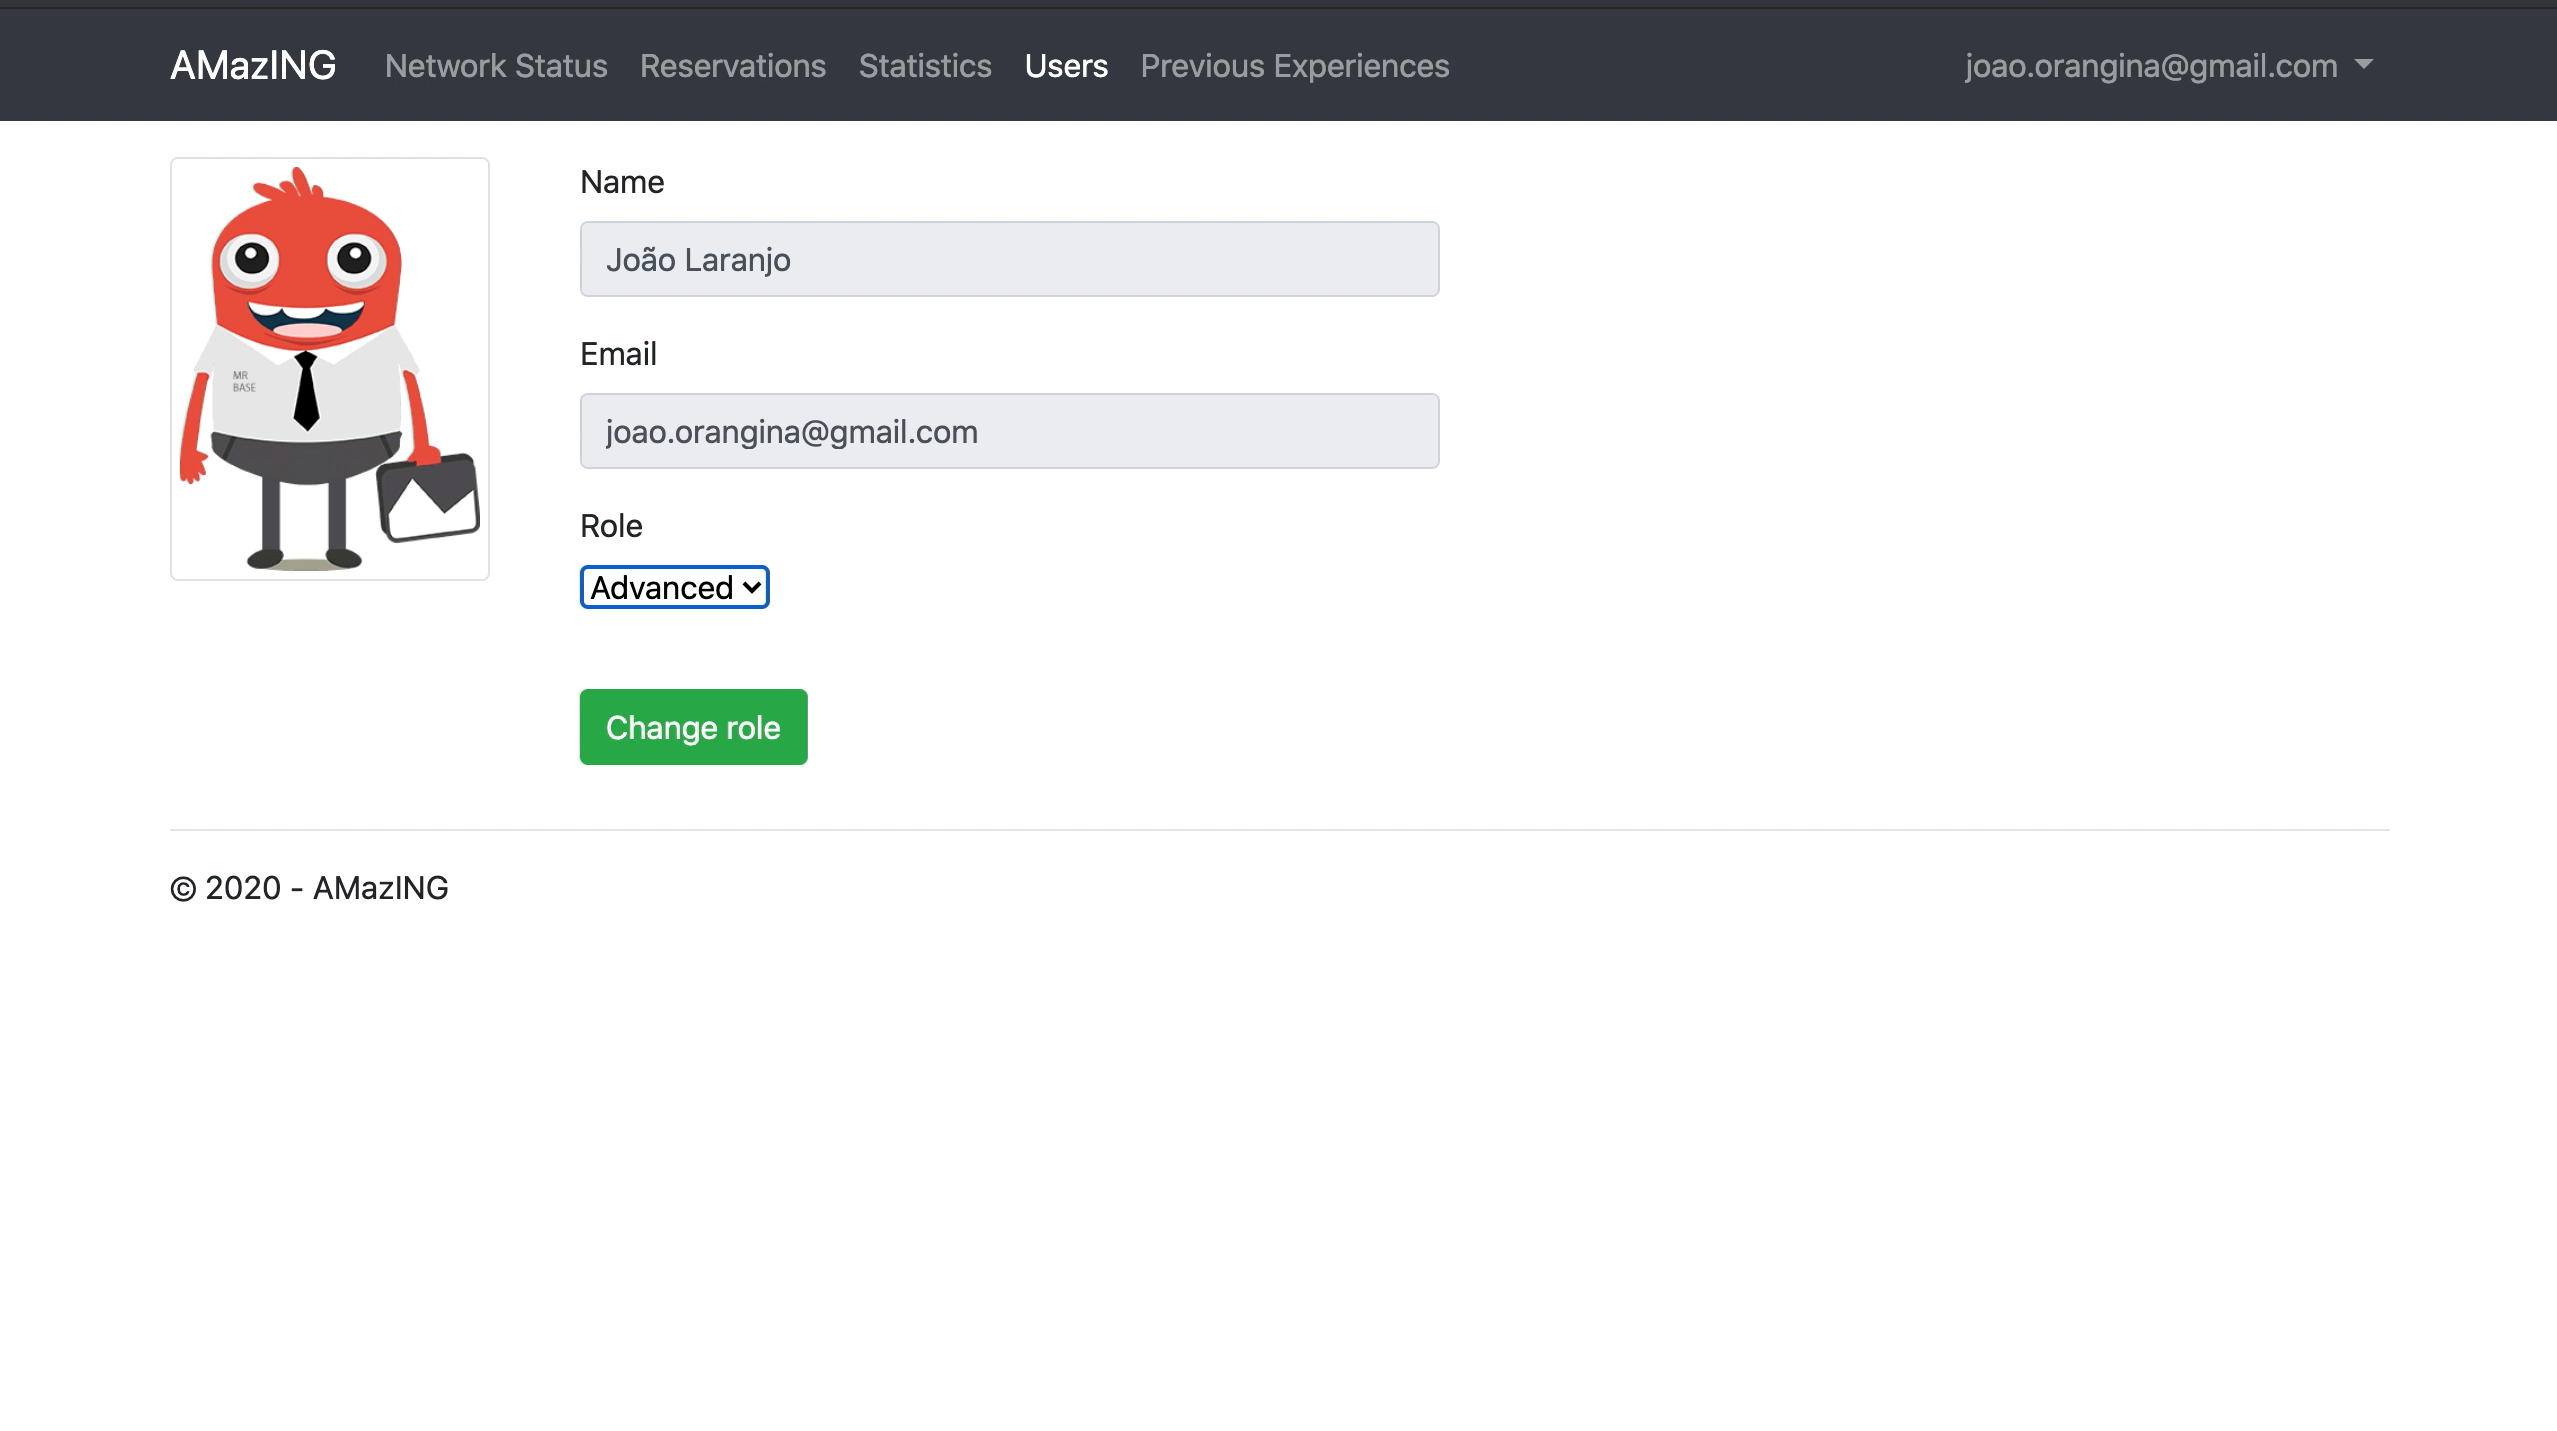
\includegraphics[width=0.9\textwidth]{images/change_user_role.png}
    \caption{Alteração de categoria de utilizador}
    \label{fig:seeprofile}
\end{figure}

\section{Nós/APUs}
Cada nó é considerado um componente distinto e, embora possam comunicar entre si, cada um é responsável pelos seus próprios processos. Como referido anteriormente, cada nó é constituído por três interfaces físicas, uma para controlo e duas para dados. Para além disso, existem também duas interfaces wireless para dados.\newline\\
Em cada nó é iniciado um servidor Flask, permitindo a comunicação com o backend e o frontend. As interações do utilizador são enviadas através de pedidos HTTP para o servidor Flask de backend, que encaminha o pedido para nó respectivo através da interface de controlo.\newline\\
Foram instaladas ferramentas como:
\begin{itemize}
    \item dnsmasq - Permite cache DNS e funciona como servidor DHCP;
    \item wpa\_supplicant - Implementa protocolos de segurança e permite ligações WPA;
    \item iperf3 - Ferramenta utilizada para medir e configurar os desempenhos da rede;
    \item Através delas, foi possível a programação de instruções que tornassem um nó num router, access point, servidor ou cliente.
\end{itemize}
Em resumo, sempre que pretendemos receber informação ou enviar uma instrução para um determinado nó, é feita uma chamada ao servidor Flask que inicia a execução de uma determinada instrução. 

\section{Deployment}
Para o  deployment de todo o projeto utilizou-se como  recurso os containers do Docker, através da criação de Dockerfiles. Cada componente do sistema tem o seu Dockerfile, sendo este utilizado através de comandos bash que lançam as respetivas instâncias (consultar anexo \ref{app:deploybash}).

\subsection{PostgreSQL}
Para a instanciação deste container, foi desenvolvido um script bash (consultar anexo \ref{app:postgre}) que permite a replicação da instalação desta base de dados e cuja a imagem se encontra no DockerHub.

\subsection{Flask API}
De forma a que fosse possível instanciar este container, foi desenvolvido um Dockerfile (consultar anexo \ref{app:flask}) que permite a criação de uma nova instância da API Flask através do código mais atual, desde que este possua as variáveis de ambiente definidas, estas pode ser colocadas dentro de um ficheiro .env ou fazendo exportação através da bash.

\subsection{Django}
Por forma a instanciar este container, foi desenvolvido um Dockerfile (consultar anexo \ref{app:django}) que permite que seja criada uma nova instância do Frontend através do código mais atual. Para que isto aconteça, basta estar dentro da pasta que contém o código do Frontend e executar o script de instalação (consultar anexo \ref{app:deploybash}).\newline
É de salientar que este script possui duas versões, uma versão que permite ao programador utilizar o Django em modo de debug (útil para quando está a fazer debug) e uma versão que permite colocar em modo de produção, bastando comentar ou descomentar a linha da versão que quer, tal como é referido nos comentários apresentados neste Dockerfile. É imporante salientar que também neste caso é necessário definir variáveis de ambiente sendo que estas podem ser exportadas através da bash ou colocadas num ficheiro .env.

\subsection{WebSSH}
O WebSSH, tal como mencionado anteriormente, é um servidor baseado numa biblioteca Python. Deste modo, para que seja possível fazer o deployment, basta existir um Dockerfile (consultar anexo \ref{app:webssh}) que tenha como função instanciar um container de Python. Após a instalação da dependência, é lançada a biblioteca na forma de serviço.
\newpage
\hfill\break
